% !Mode:: "TeX:UTF-8"
%% 请使用 XeLaTeX 编译本文.
\documentclass[forprint, AutoFakeBold, AutoFakeSlant ]{WHUExperiment}
%---------------------这里添加所需的命令--------------------------------
\lstdefinelanguage{json}{ % 定义json代码高亮
    morestring=[d]",
    stringstyle=\color{red!50!brown},
    showstringspaces=false,
    literate=
     *{0}{{{\color{Gray}0}}}{1}
      {1}{{{\color{Gray}1}}}{1}
      {2}{{{\color{Gray}2}}}{1}
      {3}{{{\color{Gray}3}}}{1}
      {4}{{{\color{Gray}4}}}{1}
      {5}{{{\color{Gray}5}}}{1}
      {6}{{{\color{Gray}6}}}{1}
      {7}{{{\color{Gray}7}}}{1}
      {8}{{{\color{Gray}8}}}{1}
      {9}{{{\color{Gray}9}}}{1}
      {:}{{{\color{Purple}{:}}}}{1}
      {,}{{{\color{Purple}{,}}}}{1}
      {\{}{{{\color{BlueGreen}{\{}}}}{1}
      {\}}{{{\color{BlueGreen}{\}}}}}{1}
      {[}{{{\color{BlueGreen}{[}}}}{1}
      {]}{{{\color{BlueGreen}{]}}}}{1},
}

%--------------------------------------------------------------------------
\makeatletter
\def\BState{\State\hskip-\ALG@thistlm}
\makeatother
\begin{document}
\nocite{*} % 允许在没有显式引用的情况下生成参考文献列表
%-----------------------------------------------------------------------------

%%%%%%% 下面的内容, 据实填空.

\Ccoursename{计算机科学与工程学院} % 映射为学院名称
\Cmajor{软件工程} % 专业名称
\title{基于 Vulkan 的实时光线追踪混合渲染器实现} % 论文题目
\Etitle{Implementation of a Real-time Ray Tracing Hybrid Renderer Based on Vulkan} % 英文题目
\author{向晨} % 学生姓名
\CstudentNum{20221889} % 学号
\Csupervisor{韩强} % 校内指导教师
\CsupervisorAnother{（无）} % 企业/校外指导教师 
\date{二〇二六年五月十五日} % 论文提交时间

%-----------------------------------------------------------------------------

\pdfbookmark[0]{封面}{title}         % 封面页加到 pdf 书签
\maketitle
\frontmatter
\pagenumbering{Roman}              % 正文之前的页码用大写罗马字母编号
%-----------------------------------------------------------------------------
% !Mode:: "TeX:UTF-8"

\makeatletter % 允许在正文中使用带有 @ 的内部变量

%%% 此部分需要自行填写: 中文摘要及关键词 

%%%---- 1. 诚信承诺书 ------------------------------------%
\newpage
\thispagestyle{empty}
\bgroup
  \setlength{\parindent}{0em}
  \linespread{1.5}\selectfont

  \vspace*{1em}
  {\centering \songti\zihao{3} 北方民族大学本科毕业论文（设计）诚信承诺书 \par}

  \vspace{1.5em}

  \noindent
  \begin{tabular}{|p{0.18\textwidth}|p{0.28\textwidth}|p{0.15\textwidth}|p{0.28\textwidth}|}
  \hline
  \centering 学生姓名 & \centering \@author & \centering 年级 & \centering\arraybackslash 2022 级 \\
  \hline
  \centering 所学专业 & \centering \the\Cmajor & \centering 学号 & \centering\arraybackslash \the\CstudentNum \\
  \hline
  \centering 所在学院 & \multicolumn{3}{c|}{\the\Ccoursename} \\
  \hline
  \multicolumn{4}{|p{\dimexpr\textwidth-2\tabcolsep-2\arrayrulewidth\relax}|}{
    \def\arraystretch{1.5}
    
    \vspace{1em}
    {\centering \heiti\zihao{3} 学生承诺 \par}
    
    \vspace{1.5em}
    {
      \songti\zihao{4} 
      \setlength{\parindent}{2em}
      \noindent \textbf{本人郑重承诺和声明：}\par
      \indent 我承诺在毕业论文（设计）过程中严格遵守学校有关规定，在指导教师的安排与指导下独立完成所规定的毕业论文（设计）工作，决不弄虚作假，不请别人代做毕业论文（设计）或抄袭别人的成果。所撰写的毕业论文或毕业设计是在指导老师的指导下自主完成，文中所有引文或引用数据、图表均注解并说明来源，本人愿意为由此引起的后果承担责任。\par
    }
    
    \vspace{5em}
    \begin{flushright}
      {\songti\zihao{4} 
      学生（签名）：\makebox[8em]{\hrulefill} \hspace{2em} \par
      \vspace{1.5em}
      2026 年 05 月 \hspace{1em} 日 \hspace{2em} \par
      }
    \end{flushright}
    \vspace{1.5em}
  } \\
  \hline
  \end{tabular}

  \vfill

  \begin{flushright}
    {\zihao{4} 教务处制}
  \end{flushright}
\egroup
\clearpage

%%======摘要===========================%
\begin{cnabstract}
\thispagestyle{empty}

在现代实时计算机图形学中，传统的纯光栅化渲染在处理全局光照、精确物理软阴影与复杂镜面反射时存在固有的物理局限性，而离线级别的纯路径追踪又难以满足交互式应用的实时帧率需求。针对这一“画质与算力”的矛盾，本文基于现代显式图形 API Vulkan 1.3，设计并实现了一套工业级的高性能实时光线追踪混合渲染引擎。

本文的核心工作包括三个方面。首先，针对 Vulkan 繁琐的显存状态同步痛点，设计了数据驱动的 Render Graph 调度架构，通过有向无环图的拓扑分析实现了管线屏障的自动推导与显存复用优化。其次，构建了高效的混合光照管线，将几何光栅化与硬件光线追踪深度解耦。在延迟渲染 G-Buffer 的基础上，结合偏导数面法线偏移与 Ray Query 扩展实现了精准无伪影的软硬阴影，并利用 RT Pipeline 全面求解 Cook-Torrance 微面元模型，完成了基于物理（PBR）的多次镜面反射计算。最后，针对 1 SPP 极低采样率带来的蒙特卡洛高频噪声，完整集成了时空方差导向滤波（SVGF）降噪系统。通过几何运动矢量的时域历史重投影与动态方差引导的多轮 A-Trous 空域滤波，成功实现了高保真度的抗噪平滑处理。

性能测试与效果分析表明，本系统在 2K 原生分辨率下，能够以实时的性能开销（稳定大于 60 帧）输出平滑且物理正确的照片级渲染画面。本文的研究验证了以 Render Graph 为底座、结合光栅化、硬件光追与 SVGF 降噪的混合架构在现代底层图形引擎开发中的高效性与工程可行性。

\end{cnabstract}
\par
\vspace*{2em}

%%%%--  关键词 -----------------------------------------%%%%%%%%
\cnkeywords{Vulkan；实时光线追踪；混合渲染；Render Graph；基于物理的渲染 (PBR)；SVGF 降噪}

\newpage
%%%---- 3. 英文摘要 ------------------------------------%
\begin{enabstract}
\thispagestyle{empty}

In modern real-time computer graphics, traditional pure rasterization rendering has inherent physical limitations when dealing with global illumination, precise physical soft shadows, and complex specular reflections, while offline-level pure path tracing is difficult to meet the real-time frame rate requirements of interactive applications. To address this contradiction between "image quality and computing power", this paper designs and implements an industrial-grade high-performance real-time ray tracing hybrid rendering engine based on the modern explicit graphics API Vulkan 1.3.

The core work of this paper includes three aspects. First, a data-driven Render Graph scheduling architecture was designed to address the tedious GPU memory state synchronization pain points of Vulkan. Through topological analysis of a directed acyclic graph, the automatic derivation of pipeline barriers and optimization of memory reuse were achieved. Second, an efficient hybrid lighting pipeline was constructed to deeply decouple geometric rasterization from hardware ray tracing. Based on deferred rendering G-Buffer, combined with derivative face normal offset and Ray Query extension, precise and artifact-free soft and hard shadows were implemented. Furthermore, the RT Pipeline was used to comprehensively solve the Cook-Torrance microfacet model, completing multi-bounce specular reflection calculations based on physics (PBR). Finally, addressing the high-frequency Monte Carlo noise caused by the extremely low sampling rate of 1 SPP, a complete Spatiotemporal Variance-Guided Filtering (SVGF) denoising system was integrated. High-fidelity anti-noise smoothing was successfully achieved through temporal history reprojection of geometric motion vectors and multi-round spatial A-Trous filtering guided by dynamic variance.

Performance tests and effectiveness analysis show that this system can output smooth and physically correct photo-realistic rendering results with real-time performance overhead (stable above 60 FPS) at 2K native resolution. This research verifies the efficiency and engineering feasibility of a hybrid architecture based on Render Graph, combining rasterization, hardware ray tracing, and SVGF denoising in modern low-level graphics engine development.

\end{enabstract}
\par
\vspace*{2em}

\enkeywords{Vulkan; Real-time Ray Tracing; Hybrid Rendering; Render Graph; Physically Based Rendering (PBR); SVGF Denoising}

\makeatother % 恢复 @ 的原始定义    % 加入摘要, 申明.
%==========================把目录加入到书签==============================%%%%%%


\tableofcontents
\thispagestyle{empty}
\addtocontents{toc}{\protect\thispagestyle{empty}}




\mainmatter %% 以下是正文
%%%%%%%%%%%%%%%%%%%%%%%%%%%--------main matter-------%%%%%%%%%%%%%%%%%%%%%%%%%%%%%%%%%%%%
\pagestyle{plain}
\linespread{1.5}\selectfont
\songti \zihao{-4}

%此处书写正文-------------------------------------------------------------------------------------

\chapter{绪论}

\section{研究背景及意义}

近三十年来，实时计算机图形学领域长期由光栅化（Rasterization）技术主导。光栅化凭借其卓越的并行计算效率，通过将三维几何顶点投影至二维屏幕空间并进行片元插值，能够在有限的硬件算力下实现高分辨率与高帧率的图像渲染。然而，光栅化本质上属于基于局部几何信息的启发式算法，难以精确模拟物理世界中光线在三维空间内的全局传输与多次反弹路径。因此，在处理全局光照（Global Illumination, GI）、基于物理的软阴影（Soft Shadows）以及多重粗糙镜面反射（Glossy Reflections）等复杂光学现象时，传统光栅化管线通常只能依赖预计算或屏幕空间经验近似算法。例如，使用屏幕空间环境光遮蔽（SSAO）来模拟暗角，使用级联阴影贴图（CSM）来计算硬阴影，以及使用屏幕空间反射（SSR）来模拟镜面效果。这些近似方案在复杂场景中极易引入明显的视觉伪影（Visual Artifacts），如 SSR 导致的屏幕外信息缺失与反射断裂。此外，随着现代数字娱乐产业对渲染真实感需求的日益提升，堆叠各类屏幕空间特效往往会导致渲染管线复杂度剧增，系统维护成本急剧上升。

随着图形硬件算力的持续突破以及 Vulkan Ray Tracing、DirectX Raytracing (DXR) 等现代图形 API 扩展的标准化，硬件加速的实时光线追踪（Hardware-Accelerated Ray Tracing）技术已正式步入实时渲染的舞台。该技术通过在硬件层面加速边界体积层次结构（Bounding Volume Hierarchy, BVH）的遍历与射线-三角形求交测试，能够精确求解渲染方程（Rendering Equation），从而生成具有照片级真实感（Photorealism）的图像。然而，受限于当前图形处理器（GPU）的显存带宽与核心算力瓶颈，在复杂的高分辨率实时交互场景中，若直接采用与离线影视渲染相同的纯路径追踪（Path Tracing）算法，每像素需要发射数千条光线，这与实时渲染严格的 $16.6$ 毫秒（60 FPS）帧时间预算存在巨大的性能鸿沟。

面对这一性能与画质的尖锐矛盾，混合渲染（Hybrid Rendering）架构应运而生。混合渲染的核心思想是“扬长避短”：利用光栅化极高的可见性判定效率生成包含场景几何与材质属性的几何缓冲（G-Buffer），随后利用硬件光线追踪在 G-Buffer 的表面属性基础上发射极少量（通常为 1 SPP，即每像素 1 条射线）光线，专门用于求解光栅化难以处理的阴影、反射和间接光照信号。然而，1 SPP 的极低采样率必然会导致渲染结果呈现出剧烈的蒙特卡洛随机噪声。因此，必须通过先进的时空降噪算法（Spatiotemporal Denoising）与时间抗锯齿技术（Temporal Anti-Aliasing, TAA）来修复低采样率带来的信噪比缺失。本文正是在此背景下，基于 Vulkan API 深入探索并实现了一套具备工业级降噪与抗锯齿能力的实时光线追踪混合渲染系统。

\section{国内外研究现状与发展}

实时渲染技术的发展史，本质上是对物理世界光照规律不断逼近的演进史。当前国内外的研究现状主要集中在以下三个技术脉络：

\subsection{实时渲染框架的演进}
早期的实时渲染引擎主要采用前向渲染（Forward Rendering）管线。前向渲染在处理每一个几何图元时，都会立即遍历场景中的所有光源进行光照计算。这种几何绘制与光照计算高度耦合的模式，导致其在面对多光源、高复杂度场景时，由于大量不可见片元被重复计算（Overdraw），性能会急剧下降。

为了解决多光源的性能瓶颈，延迟渲染（Deferred Rendering）被提出并广泛应用于现代 3D 引擎（如 Unreal Engine、Unity）中。延迟渲染通过引入几何缓冲（G-Buffer），将几何处理阶段与光照计算阶段完全分离。在几何阶段，系统仅将可见图元的反照率（Albedo）、法线（Normal）、材质粗糙度（Roughness）和深度（Depth）等属性写入 G-Buffer；在光照阶段，则直接利用 G-Buffer 中的物理属性进行全屏的光照合成。这种架构将光照计算的复杂度从“光源数量 $\times$ 几何图元数量”降低为“光源数量 $\times$ 屏幕像素数量”，极大提升了复杂光照环境下的渲染效率。然而，延迟渲染也带来了显存带宽开销大、难以处理半透明物体以及与传统多重采样抗锯齿（MSAA）不兼容等局限性。

\subsection{光线追踪技术的发展}
光线追踪技术最早由 Turner Whitted 于 1980 年提出（Whitted-style Ray Tracing），奠定了利用递归射线追踪实现镜面反射与折射的理论基础。1986 年，Kajiya 提出了著名的渲染方程（Rendering Equation），并将蒙特卡洛积分引入光线追踪，形成了路径追踪（Path Tracing）算法，首次在数学上统一了全局光照的求解模型。

长期以来，受限于庞大的计算量，该技术仅应用于影视特效等离线渲染领域。直到 2018 年，NVIDIA 发布了包含 RT Core 专用硬件加速单元的 RTX 系列显卡，Khronos Group 随后推出了 \texttt{VK\_KHR\_ray\_tracing} 扩展集，实时光线追踪才在底层硬件和 API 层面成为可能。目前，国内外顶尖工业界的主流做法均是结合光栅化与光追的混合架构，但如何在极低的光线预算下最大化光追画质，仍是学术界和工业界共同探索的热点方向。

\subsection{实时降噪与抗锯齿技术的发展}
在混合渲染管线中，降噪（Denoising）与抗锯齿（Anti-Aliasing）是决定最终画质的核心环节。
\begin{itemize}
    \item \textbf{抗锯齿技术}：由于延迟渲染无法高效使用硬件 MSAA，早期工业界多采用快速近似抗锯齿（FXAA）或次像素形态抗锯齿（SMAA）等纯空间后处理算法，但这些算法无法解决高频几何边缘的时间闪烁问题。近年来，时间抗锯齿（Temporal Anti-Aliasing, TAA）逐渐成为主流。TAA 通过在投影矩阵中引入 Halton 亚像素抖动（Sub-pixel Jitter），结合运动矢量（Motion Vector）将多帧的历史采样结果进行指数滑动平均（EMA），以极低的性能开销实现了媲美超采样（SSAA）的抗锯齿质量。
    \item \textbf{降噪技术}：针对 1 SPP 极低样本率下的蒙特卡洛噪声，传统的空间降噪算法（如双边滤波或 Edge-avoiding \`{A}-Trous 小波滤波）在强力抹平噪声的同时，往往会严重模糊几何边界与纹理细节。2017 年，Schied 等人提出了时空方差导向滤波（SVGF, Spatiotemporal Variance-Guided Filtering）算法。该算法开创性地将时间域的历史累积与空间域的 \`{A}-Trous 滤波相结合，通过估算局部时间方差（Temporal Variance）来动态调整空间滤波的边缘停止权重（Edge-stopping weights）。SVGF 成功实现了在保留高频几何细节的同时抹平低频噪声，目前已成为业界处理实时光追信号的标准基线算法。
\end{itemize}

\section{本文主要研究内容与贡献}

本文针对现代实时渲染中高画质与高性能难以兼顾的问题，基于 Vulkan 图形 API 设计并实现了一套完整的实时光线追踪混合渲染系统。针对工业界开发中的痛点，本文在系统架构、混合管线设计以及时空信号处理上进行了深度优化。主要工作与贡献如下：

\begin{enumerate}
    \item \textbf{设计并实现了基于 Render Graph 的渲染图架构}：针对 Vulkan 显式 API 中显存屏障（Memory Barrier）、图像布局转换（Image Layout Transition）和生命周期管理极其繁琐且易出错的痛点，实现了一套自动化的渲染图调度系统。该系统能够根据资源的读写约束和有向无环图（DAG）拓扑排序，在运行时自动推导管线的同步状态，极大提升了混合渲染管线的扩展性与资源复用率。
    
    \item \textbf{构建了高效的混合物理光照渲染管线}：结合延迟渲染框架，在 G-Buffer 的基础上实现了基于物理的渲染（PBR）光照计算。针对不同的光照特征灵活采用了底层光追技术：利用 Ray Query 结合几何偏导数（Derivative Face Normal）实现无自相交伪影的精确软硬阴影；利用 RT Pipeline（Raygen, Miss, ClosestHit）实现硬件加速的粗糙镜面反射与漫反射全局光照（GI）。
    
    \item \textbf{实现了基于 SVGF 的工业级时空降噪系统}：针对 1 SPP 光追信号的严重噪声问题，实现并优化了 SVGF 降噪数据流。本文深入解决了 SVGF 算法在实际工程中遇到的多项隐蔽缺陷：包括修正 Reversed-Z（反转 Z 缓冲）非线性深度导致的边缘判定失效问题，以及提出在光追着色器中解耦反照率（Demodulate Albedo），从而避免空间滤波对纹理细节的错误涂抹。
    
    \item \textbf{集成了高精度的 TAA 时间抗锯齿技术}：基于 Halton 序列实现了亚像素抖动系统。为解决 TAA 重投影过程中的历史错位与屏幕物理震动问题，本文在着色器底层推导并实现了严谨的抖动补偿公式（Jitter Compensation），并通过 AABB 颜色方差裁剪（Variance Clipping）有效消除了动态场景下的鬼影（Ghosting）现象，最终输出了极其平滑、稳定的照片级渲染画面。
\end{enumerate}

\section{论文结构安排}

本文的组织结构如下：
\begin{itemize}
    \item \textbf{第一章 绪论}：阐述课题的研究背景、意义及国内外发展现状，并总结本文的主要研究内容与贡献。
    \item \textbf{第二章 实时混合渲染理论基础}：详细介绍基于物理的渲染（PBR）材质模型、Vulkan API 的核心机制与显式同步理论，以及硬件光线追踪加速结构（BVH）的基本原理。
    \item \textbf{第三章 基于 Render Graph 的渲染器架构设计}：详细论述渲染图的节点抽象、虚拟资源池管理、以及 Vulkan 状态屏障的自动推导算法与乒乓轮换（Ping-Pong）机制的工程实现。
    \item \textbf{第四章 混合光照管线的核心设计与实现}：重点分析 G-Buffer 延迟管线构建、微表面 BRDF 物理光照合成逻辑，以及 Ray Query 与 RT Pipeline 在具体光影效果中的应用与优化。
    \item \textbf{第五章 基于时空域的抗锯齿与降噪算法实现}：深入剖析蒙特卡洛噪声与锯齿的形成原理。详细推导 TAA 的亚像素重投影数学模型，并全面讲解 SVGF 算法中历史累积、方差估算与 \`{A}-Trous 空域滤波的实现细节及工业级防坑指南。
    \item \textbf{第六章 渲染效果展示与性能分析}：通过丰富的对比实验图展示混合渲染器的最终画面质量，对比光栅化与光线追踪的视觉差异，并通过 GPU 耗时统计验证系统在不同负载下的实时性能。
    \item \textbf{第七章 总结与展望}：对全文的核心工作进行总结，客观分析当前系统的局限性，并对引擎未来可能的优化方向（如 ReSTIR 等新兴算法）进行展望。
\end{itemize}
\chapter{实时混合渲染理论基础}

构建高保真的实时光线追踪混合渲染器，不仅是一项复杂的软件工程任务，更需要跨越计算机图形学基础、物理光学、概率论数值积分方法、底层图形硬件架构以及信号处理理论等多个维度的知识壁垒。本章将从传统的经典光栅化渲染管线出发，系统性地阐述坐标变换与光栅化的数学基础及其固有的物理局限性；随后详细解析基于物理的渲染（PBR）核心数学模型、蒙特卡洛积分理论与 Vulkan 图形 API 的显式状态管理机制；最后深入探讨硬件级光线追踪的底层运行机制。这些跨学科的理论体系将为后续章节的混合管线架构设计、光照算法实现以及时空降噪网络的构建提供完备且严谨的理论支撑。

\subsection{三维坐标系与空间变换数学模型}

现代光栅化图形管线是一条高度优化的单向数据流流水线，其首要任务是将三维空间中的几何顶点准确投射到二维屏幕上。由于传统的三维向量无法通过单一的线性矩阵乘法同时表示旋转、缩放与平移，图形学引入了齐次坐标（Homogeneous Coordinates），将三维坐标 $(x, y, z)$ 升维至四维 $(x, y, z, w)$。基于齐次坐标的仿射变换（Affine Transformation）构成了光栅化管线的数学基石。 

整个顶点映射过程需要经历严密的线性代数矩阵变换序列，即经典的 MVP 变换（Model-View-Projection）以及后续的视口映射：

\begin{enumerate}
    \item \textbf{模型变换（Model Transformation）}：将顶点从物体的局部坐标系（Local Space）变换至世界坐标系（World Space）。该变换矩阵 $M_{model}$ 通常由缩放矩阵 $S$、旋转矩阵 $R$ 与平移矩阵 $T$ 复合而成，即 $M_{model} = T \cdot R \cdot S$。以平移矩阵为例，其齐次形式定义为：
    \begin{equation}
    T(t_x, t_y, t_z) = 
    \begin{bmatrix}
    1 & 0 & 0 & t_x \\
    0 & 1 & 0 & t_y \\
    0 & 0 & 1 & t_z \\
    0 & 0 & 0 & 1
    \end{bmatrix}
    \end{equation}

    \item \textbf{视图变换（View Transformation）}：将世界坐标系变换至以摄像机为原点的视图坐标系（View Space / Camera Space）。假设摄像机的位置为 $\vec{e}$，观察目标点为 $\vec{t}$，向上的参考向量为 $\vec{u}$。首先构建摄像机坐标系的标准正交基：前向向量 $\vec{f} = \frac{\vec{t} - \vec{e}}{||\vec{t} - \vec{e}||}$，右向量 $\vec{r} = \frac{\vec{f} \times \vec{u}}{||\vec{f} \times \vec{u}||}$，以及真正的上向量 $\vec{u'} = \vec{r} \times \vec{f}$。视图矩阵 $M_{view}$ 可推导为先平移后旋转的逆变换矩阵：
    \begin{equation}
    M_{view} = 
    \begin{bmatrix}
    r_x & r_y & r_z & 0 \\
    u'_x & u'_y & u'_z & 0 \\
    -f_x & -f_y & -f_z & 0 \\
    0 & 0 & 0 & 1
    \end{bmatrix}
    \begin{bmatrix}
    1 & 0 & 0 & -e_x \\
    0 & 1 & 0 & -e_y \\
    0 & 0 & 1 & -e_z \\
    0 & 0 & 0 & 1
    \end{bmatrix}
    \end{equation}

    \item \textbf{投影变换（Projection Transformation）}：引入透视除法以产生“近大远小”的真实深度感。顶点被变换至齐次裁剪空间（Clip Space）。在该空间下，硬件将自动剔除处于视锥体（Frustum）之外的几何图元。标准的透视投影矩阵 $M_{proj}$ 定义为：
    \begin{equation}
    M_{proj} = 
    \begin{bmatrix}
    \frac{1}{aspect \cdot \tan(fov/2)} & 0 & 0 & 0 \\
    0 & \frac{1}{\tan(fov/2)} & 0 & 0 \\
    0 & 0 & -\frac{f+n}{f-n} & -\frac{2fn}{f-n} \\
    0 & 0 & -1 & 0
    \end{bmatrix}
    \end{equation}
    其中 $fov$ 为视场角（Field of View），$aspect$ 为屏幕宽高比，$n$ 和 $f$ 分别为近剪裁面与远剪裁面的距离。注意矩阵的最后一行变成了 $(0, 0, -1, 0)$，这是为了将摄像机空间下的 $-z$ 值保存至齐次坐标的 $w$ 分量中。

    \item \textbf{透视除法与标准化设备坐标（NDC）}：在投影变换之后，GPU 硬件会自动执行透视除法（Perspective Division），即将顶点的四维齐次坐标统一除以其 $w$ 分量：
    \begin{equation}
    P_{ndc} = \left( \frac{x_{clip}}{w_{clip}}, \frac{y_{clip}}{w_{clip}}, \frac{z_{clip}}{w_{clip}} \right)
    \end{equation}
    此时，所有可见的三维顶点被严格压缩至一个边长为 $2$ 的标准立方体中，即 $x, y \in [-1, 1]$（Vulkan 中 $z \in [0, 1]$），形成标准化设备坐标（Normalized Device Coordinates, NDC）。

    \item \textbf{视口变换（Viewport Transformation）}：最后，系统将 NDC 坐标映射到实际的二维屏幕像素矩阵上。设屏幕宽度为 $W$，高度为 $H$，屏幕坐标系原点位于左上角，则视口变换公式为：
    \begin{equation}
    x_{screen} = \frac{x_{ndc} + 1}{2} \cdot W, \quad y_{screen} = \frac{y_{ndc} + 1}{2} \cdot H
    \end{equation}
    至此，三维空间中的几何顶点彻底完成了向二维像素物理地址的转换，为后续的重心坐标插值与片元着色奠定了基础。
\end{enumerate}

\subsection{图元装配与重心坐标光栅化}

顶点经过透视除法映射到标准化设备坐标（NDC）并完成视口变换后，硬件将分散的顶点组装为具有拓扑关系的三角形图元。随后，光栅化器（Rasterizer）接管流程，将连续的二维三角形离散化为屏幕像素网格上的片元（Fragments）。这一阶段包含三个极其严密的数学判定与插值过程：

\begin{enumerate}
    \item \textbf{图元装配与背面剔除（Backface Culling）}：
    在三维模型中，绝大多数封闭网格的背面是对摄像机不可见的。为了节省光栅化算力，硬件会根据三角形在屏幕空间的顶点环绕顺序（Winding Order，如逆时针为正面）进行剔除。设三角形的三个屏幕顶点为 $V_0(x_0, y_0)$、$V_1(x_1, y_1)$ 和 $V_2(x_2, y_2)$，通过计算边向量的二维叉积，可以得到有向面积的两倍：
    \begin{equation}
    S = (x_1 - x_0)(y_2 - y_0) - (x_2 - x_0)(y_1 - y_0)
    \end{equation}
    若 $S \le 0$，则表示该三角形背向摄像机或退化为一条线，硬件将直接将其丢弃。

    \item \textbf{边方程（Edge Equations）与像素相交测试}：
    对于通过剔除的三角形，光栅化器需要遍历屏幕像素（通常结合分块包围盒优化），判断像素中心 $P(x, y)$ 是否位于三角形内部。现代 GPU 广泛采用 Juan Pineda 于 1988 年提出的边方程算法。对于有向边 $V_i \to V_j$，定义边函数 $E_{ij}(x, y)$ 为：
    \begin{equation}
    E_{ij}(x, y) = (x - x_i)(y_j - y_i) - (y - y_i)(x_j - x_i)
    \end{equation}
    当且仅当像素 $P(x, y)$ 对于三角形的三条边均满足 $E_{01} \ge 0$、$E_{12} \ge 0$ 和 $E_{20} \ge 0$（或同为负）时，该像素被判定为位于三角形内部，从而生成一个有效片元。

    \item \textbf{重心坐标（Barycentric Coordinates）的几何推导}：
    在确认像素位于三角形内部后，系统需要利用重心坐标 $(\alpha, \beta, \gamma)$ 在三角形内部平滑插值顶点的各种属性（如法线、UV 坐标、颜色等）。重心坐标本质上是面积比，对于点 $P(x, y)$，其系数可通过边函数的值直接求得：
    \begin{equation}
    P(x, y) = \alpha V_0 + \beta V_1 + \gamma V_2
    \end{equation}
    \begin{equation}
    \alpha = \frac{E_{12}(x, y)}{E_{12}(x_0, y_0)}, \quad \beta = \frac{E_{20}(x, y)}{E_{20}(x_1, y_1)}, \quad \gamma = \frac{E_{01}(x, y)}{E_{01}(x_2, y_2)}
    \end{equation}
    其中，$\alpha + \beta + \gamma = 1$。
    
    \item \textbf{透视校正插值（Perspective-Correct Interpolation）}：
    在早期的三维渲染中，直接利用上述屏幕空间的重心坐标对顶点属性 $I$（如纹理 UV）进行线性插值（$I_p = \alpha I_0 + \beta I_1 + \gamma I_2$）会导致严重的视觉透视扭曲。这是因为投影变换是非线性的，屏幕空间上的均匀步进并不对应三维物理空间中的均匀步进。
    为了实现物理正确的插值，现代管线引入了透视校正机制。真正的插值必须在齐次裁剪空间的 $w$ 分量（代表深度）的辅助下完成。首先对 $1/w$ 进行屏幕空间线性插值以求得当前像素的真实深度权重：
    \begin{equation}
    \frac{1}{w_p} = \alpha \frac{1}{w_0} + \beta \frac{1}{w_1} + \gamma \frac{1}{w_2}
    \end{equation}
    随后，对目标属性 $I$ 除以 $w$ 后的值进行插值，再乘以像素真实的 $w_p$：
    \begin{equation}
    I_p = w_p \left( \alpha \frac{I_0}{w_0} + \beta \frac{I_1}{w_1} + \gamma \frac{I_2}{w_2} \right)
    \end{equation}
\end{enumerate}

基于上述深度的数学推导与透视校正机制，光栅化器以极高的并行效率生成了海量准确的片元，并将其送入片元着色器（Fragment Shader）执行局部光照计算，最后利用 Z-Buffer 算法通过深度比较完成可见性测试。

\subsection{光栅化管线的物理局限性与算法妥协}
尽管光栅化极具并行计算效率，但它本质上是一种将三维空间强行投影到二维平面的“局部几何求解器”。在片元着色器计算光照时，管线仅能获取当前像素所属图元的局部属性（如法线、材质），对场景中其他几何体的存在与空间遮挡关系一无所知。因此，光栅化无法天然求解渲染方程中涉及半球空间积分的全局光照问题。为了在光栅化框架下模拟这些现象，工业界发展了大量基于图像空间（Image-Space）的近似算法，但这些算法均存在无法逾越的物理局限性：
\begin{itemize}
    \item \textbf{物理遮挡阴影（Shadows）}：传统管线必须依赖阴影贴图（Shadow Map）技术，即从光源视角预渲染一张深度图。该技术存在严重的透视走样（Perspective Aliasing）与投影走样（Projective Aliasing）。此外，为了解决离散纹理采样导致的自遮挡伪影（Shadow Acne），必须引入经验性的深度偏移（Depth Bias），但这又会引发物体悬浮的“彼得潘现象”（Peter Panning）。
    \item \textbf{镜面反射（Specular Reflections）}：纯光栅化通常依赖屏幕空间反射（Screen Space Reflection, SSR）。SSR 通过在当前的深度缓冲（Depth Buffer）上进行步进光线投射（Ray Marching）来寻找交点。由于深度缓冲仅保留了场景最表层的二维信息，当反射射线指向屏幕外（Off-screen），或目标物体被前景物体遮挡时，SSR 算法将彻底失效，导致反射画面出现突兀的断裂与大面积的信息丢失。
    \item \textbf{间接光照与全局照明（Global Illumination, GI）}：光线在物理世界中会在多个表面间发生多次反弹（Multi-bounce）。在光栅化下，由于缺乏场景的全局拓扑结构，极难实现实时的多次反弹计算。现有的屏幕空间全局光照（SSGI）或体素光照（VXGI）要么极度缺乏精度，要么面临巨大的内存与体素化开销。
\end{itemize}
综上所述，这些基于屏幕空间或预计算的经验近似算法在复杂场景中不仅会产生不可避免的视觉伪影，而且各种特效（SSR, SSAO, CSM）的堆叠导致渲染管线极度臃肿。这就从根本上确立了本课题引入硬件级光线追踪，以第一性原理（First Principles）获取物理正确光影的绝对必要性。

\section{光线追踪基本原理与发展脉络}

为了解决光栅化的全局光照缺失问题，光线追踪（Ray Tracing）技术应运而生。它从物理光学原理出发，逆向模拟了光线从光源发出、在场景表面反弹、最终进入虚拟相机的传播过程，从而在算法底层实现了真正的全局照明。

\subsection{经典光线追踪（Whitted-style Ray Tracing）}
1980 年，Turner Whitted 提出了经典的递归光线追踪算法。该算法从摄像机向屏幕每个像素发射一条初始射线（Primary Ray）。当射线与场景中的几何表面相交时，算法会立即向场景中的所有已知光源发射阴影射线（Shadow Ray）以判断是否被遮挡。 [Image of Whitted style ray tracing reflection and refraction] 
如果表面是完美的镜面或透明介质，算法会根据斯涅尔定律（Snell's Law）和反射定律，生成精确的反射射线（Reflection Ray）与折射射线（Refraction Ray），并沿这些新射线的方向进行递归追踪。局部光照强度 $I$ 可用递归公式表示为：
\begin{equation}
I = I_{local} + k_r \cdot I_{reflection} + k_t \cdot I_{refraction}
\end{equation}
其中 $k_r$ 和 $k_t$ 分别为反射与折射系数。然而，该算法的局限性在于：它仅能处理理想的光滑镜面与点光源，无法模拟自然界中普遍存在的粗糙表面模糊反射（Glossy Reflection）、面积光源产生的软阴影（Soft Shadows）以及漫反射表面间的颜色溢出（Color Bleeding）。

\subsection{路径追踪（Path Tracing）与维度灾难}
1986 年，James Kajiya 将蒙特卡洛数值积分（Monte Carlo Integration）引入图形学，正式提出了路径追踪（Path Tracing）算法。与 Whitted 算法固定发射反射/折射射线不同，路径追踪放弃了理想镜面的假设。在每次射线命中表面时，算法将表面材质的半球双向反射分布函数（BRDF）视作一个概率密度函数（PDF），并在半球空间内随机采样一个反弹方向继续追踪。

渲染方程的本质是一个无穷维的连续积分问题，传统数值积分（如梯形法则、辛普森法则）在处理此类高维积分时会遭遇“维度灾难”（Curse of Dimensionality），计算量呈指数级爆炸。而路径追踪巧妙地利用了蒙特卡洛方法的特性，其收敛速度 $O(N^{-1/2})$ 与积分维度无关。
当向每个像素发射的采样射线数量（SPP, Samples Per Pixel）趋于无穷大时，路径追踪的期望值能够无偏差（Unbiased）地收敛于物理世界的真实光照分布，奠定了现代电影级离线渲染的数学基础。但在实时渲染领域，由于极端的算力限制，本系统通常只能采用极低的采样率（如 1 SPP），这也直接导致了积分结果极度发散，表现为画面上剧烈的蒙特卡洛高频噪声。

\subsection{辐射度量学核心物理量与理论约束}
在计算机图形学中，描述光线能量及其在空间中分布的核心物理量包括：
\begin{itemize}
    \item \textbf{辐射通量（Radiant Flux, $\Phi$）}：光源在单位时间内辐射出的总能量，单位为瓦特（W）。
    \item \textbf{辐照度（Irradiance, $E$）}：单位面积 $A$ 上接收到的辐射通量，定义为 $E = \frac{d\Phi}{dA}$。
    \item \textbf{辐射亮度（Radiance, $L$）}：衡量单一光线强度的最核心物理量。定义为单位投影面积、单位立体角 $\omega$ 上的辐射通量，并需考虑表面法线 $n$ 与光线方向夹角 $\theta$ 的余弦衰减：
    \begin{equation}
    L = \frac{d^2\Phi}{d\omega dA \cos\theta}
    \end{equation}
\end{itemize}

材质对光线的反射特性由双向反射分布函数（BRDF）$f_r(p, \omega_i, \omega_o)$ 描述。一个物理正确的 BRDF 模型必须满足两大物理约束：
\begin{enumerate}
    \item \textbf{亥姆霍兹光路可逆性（Helmholtz Reciprocity）}：入射光路与反射光路相互反转时，BRDF 值必须保持不变，即 $f_r(p, \omega_i, \omega_o) = f_r(p, \omega_o, \omega_i)$。
    \item \textbf{能量守恒定律（Energy Conservation）}：表面反射出的总能量绝不能超过入射的总能量。对于法线上半球空间 $\Omega$ 内的任意入射方向，必须满足：
    \begin{equation}
    \int_{\Omega} f_r(p, \omega_i, \omega_o) (n \cdot \omega_o) d\omega_o \le 1
    \end{equation}
\end{enumerate}

\section{辐射度量学与基于物理的渲染（PBR）理论}

为了在虚拟场景中生成具有高度真实感的材质表现，本系统完全遵循工业标准的基于物理的渲染（Physically Based Rendering, PBR）工作流。PBR 的核心在于严格遵守能量守恒定律，并依托辐射度量学（Radiometry）精确量化光能的传输。

\subsection{辐射度量学核心物理量与半球积分}
在计算机图形学中，描述光线能量及其在三维空间中分布的核心物理量包括：
\begin{itemize}
    \item \textbf{辐射通量（Radiant Flux, $\Phi$）}：光源在单位时间内辐射出的总能量，单位为瓦特（W）。
    \item \textbf{辐射亮度（Radiance, $L$）}：衡量单一光线强度的最核心物理量，也是光线追踪算法在空间中实际传递的数值。定义为单位投影面积、单位立体角 $\omega$ 上的辐射通量：
    \begin{equation}
    L = \frac{d^2\Phi}{d\omega dA \cos\theta}
    \end{equation}
    \item \textbf{辐照度（Irradiance, $E$）}：单位面积 $A$ 上接收到的辐射通量。它与辐射亮度的数学关系表现为对法线上半球空间 $\Omega$ 的积分：
    \begin{equation}
    E = \int_{\Omega} L_i(\omega) \cos\theta d\omega
    \end{equation}
\end{itemize}

材质对光线的反射特性由双向反射分布函数（BRDF）$f_r(p, \omega_i, \omega_o)$ 描述。一个物理正确的 BRDF 模型必须满足两大物理约束：
\begin{enumerate}
    \item \textbf{亥姆霍兹光路可逆性（Helmholtz Reciprocity）}：入射光路与反射光路相互反转时，BRDF 值必须保持不变，即 $f_r(p, \omega_i, \omega_o) = f_r(p, \omega_o, \omega_i)$。
    \item \textbf{能量守恒定律（Energy Conservation）}：表面反射出的总能量绝不能超过入射的总能量。对于法线上半球空间 $\Omega$ 内的任意入射方向，必须满足：
    \begin{equation}
    \int_{\Omega} f_r(p, \omega_i, \omega_o) (n \cdot \omega_o) d\omega_o \le 1
    \end{equation}
\end{enumerate}

\subsection{渲染方程（The Rendering Equation）}
基于上述辐射度量学理论，计算机图形学中所有的光照计算，本质上都是在求解由 Kajiya 提出的渲染方程。对于场景中表面上的任意一点 $p$，其向观察方向 $\omega_o$ 辐射出的总光亮度 $L_o(p, \omega_o)$ 可以表示为： [Image of rendering equation hemisphere integration]
\begin{equation}
L_o(p, \omega_o) = L_e(p, \omega_o) + \int_{\Omega} f_r(p, \omega_i, \omega_o) L_i(p, \omega_i) (n \cdot \omega_i) d\omega_i
\label{eq:rendering_equation}
\end{equation}
其中，$L_e$ 为自发光项；$\Omega$ 表示法线上半球空间；$L_i$ 为来自入射方向 $\omega_i$ 的入射光亮度；$(n \cdot \omega_i)$ 遵循兰伯特余弦定律，模拟了光束截面积随入射角度变大而造成的能量密度衰减。

\subsection{Cook-Torrance 微面元模型与物理推导}
为了精确求解方程中的 BRDF 函数 $f_r$，本系统采用了广泛应用于现代渲染引擎的 Cook-Torrance 微面元模型。该模型基于 V-Cavity（V型凹槽）假设，认为宏观表面在微观尺度下由无数个法线朝向各异的光滑微小镜面（Microfacets）组成。 [Image of microfacet BRDF masking and shadowing] 其高光反射项解析式为：
\begin{equation}
f_{specular} = \frac{D(h) F(v, h) G(l, v, h)}{4 (n \cdot l)(n \cdot v)}
\end{equation}
其中，$h$ 为视线 $v$ 与光线 $l$ 的半程向量，分母中的 $4 (n \cdot l)(n \cdot v)$ 是从微观几何投影到宏观几何的物理校正因子。三大核心项的具体物理推导为：
\begin{itemize}
    \item \textbf{法线分布函数（NDF, $D$ 项）}：采用 Trowbridge-Reitz GGX 分布，决定了微表面法线 $m$ 与半程向量 $h$ 精确对齐的概率。它直接决定了高光斑的面积与粗糙度（拖尾效应），其中 $\alpha = Roughness^2$：
    \begin{equation}
    D_{GGX}(n, h, \alpha) = \frac{\alpha^2}{\pi \left( (n \cdot h)^2 (\alpha^2 - 1) + 1 \right)^2}
    \end{equation}
    \item \textbf{菲涅尔方程（Fresnel, $F$ 项）}：描述掠射角反射率攀升的物理现象。物理上，基础反射率 $F_0$ 由复折射率（Index of Refraction, IOR）的实部 $n_1, n_2$ 决定：$F_0 = \left(\frac{n_1 - n_2}{n_1 + n_2}\right)^2$。为避免复杂的实时计算，本系统采用 Schlick 近似模型：
    \begin{equation}
    F_{Schlick}(h, v, F_0) = F_0 + (1 - F_0)(1 - (h \cdot v))^5
    \end{equation}
    \item \textbf{几何遮蔽函数（Geometry, $G$ 项）}：采用 Smith 联合遮蔽函数，模拟微面元之间光线在射入时被遮挡（Shadowing）与反射时被自身遮蔽（Masking）导致的能量流失。
    \begin{equation}
    G_1(n, x, k) = \frac{n \cdot x}{(n \cdot x)(1 - k) + k}
    \end{equation}
\end{itemize}

\section{现代图形 API 与底层硬件调度架构}

光线追踪算法的高效落地，不仅依赖于严格的数学推导，更极其受制于现代图形处理器（GPU）的物理架构特性。本系统选用的 Vulkan API，正是为了最大限度地贴合底层硅片工作原理而设计的显式接口。

\subsection{SIMT 架构与线程发散（Divergence）瓶颈}
现代 GPU 采用单指令多线程（SIMT, Single Instruction Multiple Threads）的流式处理器架构。GPU 的底层计算单元以线程束（Wavefront/Warp，通常包含 32 或 64 个线程）为基本调度单位。在同一个线程束内的所有线程，必须在统一的程序计数器（Program Counter）驱动下，在相同时钟周期内执行完全相同的机器指令。 

在传统光栅化中，相邻像素通常属于同一个三角形，其着色与内存拾取逻辑高度一致，SIMT 执行效率逼近理论极限，且容易触发显存访问的全局合并（Memory Coalescing）。然而，在光线追踪中，当一束高度相干的初始光线击中不同粗糙度、不同法向的场景表面后，其反弹产生的次级射线（Secondary Rays）方向会变得极度随机散乱（Incoherent Rays）。
这种非相干射线会导致同一线程束内的指令路径出现巨大的发散（Execution Divergence）。例如，线程 A 需要遍历复杂的树结构，而线程 B 仅需简单的环境光采样，由于 SIMT 的锁步特性，线程 B 必须被硬件强制挂起（Active Mask 设为 0）以等待线程 A 完成。此外，发散的射线会导致 L1/L2 缓存的命中率（Cache Hit Rate）断崖式下跌，引发极高的显存延迟。因此，将高度相干的几何提取交由光栅化阶段统一处理（生成 G-Buffer），仅将不可避免的非相干物理计算交由光追处理的“混合渲染管线”，是对当前硬件架构的最优妥协。

\subsection{Vulkan 显式内存屏障与流水线同步}
与传统 OpenGL 驱动在后台隐式管理巨大的全局状态机不同，Vulkan 所有的渲染状态设置与指令录制由开发者显式操作至指令缓冲（Command Buffer）中。由于驱动程序剥离了冒险检测逻辑，系统必须手动插入管线内存屏障（Pipeline Memory Barrier）。
开发者必须精准定义执行依赖（Execution Dependency，即阻塞流水线中的哪几个 Stage）与内存依赖（Memory Dependency，即刷新或无效化哪些 Cache）。这种将硬件同步的底层权力下放的设计，虽大幅增加了代码复杂度，但彻底消除了单线程 CPU 提交瓶颈，直接催生了本文第三章 Render Graph 自动化并发调度架构。

\section{硬件加速光线追踪底层机制}

在纯计算着色器（Compute Shader）中执行光线追踪遍历极其耗时。本系统利用 NVIDIA RTX 系列显卡提供的 RT Core 专用硅片单元，实现了光线与几何体的极速求交计算。

\subsection{表面积启发式（SAH）与两级加速结构}
为了避免 $O(N)$ 复杂度的暴力求交，场景几何必须被组织为包围盒层级结构（Bounding Volume Hierarchy, BVH）。构建高质量 BVH 树的核心在于贪心优化表面积启发式算法（Surface Area Heuristic, SAH）。 
SAH 算法假设一条随机光线击中包围盒 $B$ 的概率与其表面积 $S(B)$ 成正比。在拆分树节点时，SAH 试图最小化光线遍历该节点的预期开销代价函数 $C$：
\begin{equation}
C = C_{trav} + \frac{S_L}{S_P} N_L C_{int} + \frac{S_R}{S_P} N_R C_{int}
\end{equation}
其中，$C_{trav}$ 为遍历节点的代价；$S_P, S_L, S_R$ 分别为父节点与左右子树的表面积；$N_L, N_R$ 为子树包含的三角形图元数量。
在 Vulkan 体系中，该加速结构被强制解耦为两级：底层加速结构（BLAS，包含极难构建的静态网格几何）与顶层加速结构（TLAS，包含轻量级的动态实例变换矩阵），从而保障了动态场景中光追加速结构的毫秒级实时更新。

\subsection{着色器绑定表（SBT）与执行范式}
本系统在 Vulkan 架构下综合利用了两种不同的光追执行范式：
\begin{enumerate}
    \item \textbf{Ray Query（内联光线查询）}：在常规的片段或计算着色器中隐式定义光线，利用 \texttt{rayQueryProceedEXT} 触发 RT Core 遍历。它在单线程内同步阻塞，无需维护复杂的内存数据结构，非常适合局部的直接光软硬阴影测试。
    \item \textbf{RT Pipeline（光线追踪专用管线）}：这是一种全新的异步状态机。它通过构建复杂的着色器绑定表（Shader Binding Table, SBT）来映射射线命中特定物体时该执行哪一段着色器代码。由 GPU 硬件自动调度并触发光线生成（RayGen）、未命中（Miss）或最近命中（ClosestHit）模块。其强大的递归调用与自定义载荷（Payload）寄存器传递能力，是本系统求解多重镜面反射的核心基石。
\end{enumerate}

\section{信号采样定理与走样原理}

在渲染管线末端，离散的数字像素重构决定了画面的最终平滑度。根据信息论中的奈奎斯特-香农采样定理（Nyquist-Shannon Sampling Theorem），为了无损还原一个连续的空间或时间信号，采样频率必须至少严格大于该信号最高频率分量的两倍（$f_{sample} > 2 f_{max}$）。

然而，在计算机图形学中，多边形几何体的锐利边界呈现为阶跃函数（Step Function），其经过傅里叶变换（Fourier Transform）后在频域上包含无穷高的空间频率。受限于物理显示器固定的像素网格分辨率（即采样频率的硬性上限），奈奎斯特极限必定被打破，从而产生了高频信号折叠至低频区段的现象，即空间走样（Spatial Aliasing，视觉上表现为锯齿狗牙）。同样，当物理相机快速移动时，时间维度的帧率采样不足也会导致高光闪烁与噪点蠕动（Temporal Aliasing）。这从纯粹的频域信号学底层，不可辩驳地确立了第五章中必须引入时间抗锯齿（TAA）多帧时域复用与前置低通滤波（Low-pass Filtering）的理论必然性。

\section{本章小结}

本章详细探讨了实时混合渲染引擎底层的跨学科理论基础体系。首先对比了传统光栅化管线坐标变换的物理局限性与光线追踪技术的全局优势；其次引入了 PBR 材质微面元模型与蒙特卡洛积分推导，不仅在数学上明确了光照的计算公式，更从概率论的方差层面上论证了降噪算法在实时渲染中的绝对必要性；随后剖析了 GPU 的 SIMT 执行瓶颈与 Vulkan 的显式内存同步机制；最后阐述了基于 SAH 代价函数的 BVH 加速结构与信号采样定理。这些严密的底层理论不仅定义了本课题“算什么”，更决定了在现代 GPU 上“怎么算”，为第三章系统架构的抽象与后续时空算法的落地奠定了坚实的技术基石。
\chapter{混合渲染系统架构设计与理论基础}

\section{混合渲染管线总体架构设计}

随着图形硬件对实时光线追踪（Real-time Ray Tracing）技术的原生支持，现代渲染引擎正从纯光栅化架构向混合渲染（Hybrid Rendering）架构演进。本系统设计的混合渲染管线旨在充分发挥光栅化在处理高频率几何覆盖（Geometry Coverage）方面的极高效率，同时利用光线追踪在解决非局部光照现象（如软阴影、多重反射、全局光照）上的物理精确性。

\subsection{混合渲染的设计哲学}
在实时渲染的性能约束下，完全基于路径追踪（Path Tracing）的方案在复杂场景中依然难以达到工业级的帧率要求。因此，本系统采用了“光栅化构建几何底座，光线追踪求解光照贡献”的核心策略。
在这种架构下，光栅化管线负责主视线（Primary Rays）的可见性判定，通过一次性的深度测试和属性插值生成高分辨率的几何缓冲（G-Buffer）；而光线追踪则专注于处理次级射线（Secondary Rays）的求交与采样，仅在关键的光照交互点（如阴影测试、镜面反射方向）发起昂贵的射线查询。这种动静结合的设计，确保了系统能够在主流消费级 GPU 上实现影视级的渲染效果。

\subsection{解耦的管线阶段与逻辑流转}
本系统的混合渲染管线被深度解耦为四个相互关联的功能阶段。在 Render Graph 的调度下，各阶段通过显式的资源依赖建立数据流转链路：

\begin{enumerate}
    \item \textbf{几何特征提取阶段（Geometry Pass）}：
    作为管线的入口，该阶段利用传统光栅化硬件单元并行处理场景顶点。其输出目标（Render Targets）不仅包含传统的可视颜色，更重要的是提取了像素级的物理特征字典。这包括但不限于：
    \begin{itemize}
        \item 编码了微表面细节的世界空间法线（Normal）；
        \item 用于反向投影的世界空间深度（Depth）；
        \item 描述材质物理属性的金属性与粗糙度参数（PBR Parameters）；
        \item 记录亚像素位移的运动矢量（Motion Vector）。
    \end{itemize}
    这些特征为后续的光线追踪阶段提供了精确的射线发射起点与方向依据。

    \item \textbf{硬件加速光照求解阶段（Ray Tracing Pass）}：
    该阶段是本系统的“物理核心”。它读取 G-Buffer 提供的几何信息，在每一帧中动态发起数十万至数百万条探测射线。系统利用 Vulkan 的加速结构（AS）对场景进行快速检索：
    \begin{itemize}
        \item \textbf{阴影计算}：沿光源方向发射射线，探测遮蔽物；
        \item \textbf{反射计算}：根据镜面反射定律和材质粗糙度，生成反射射线并追踪其在场景中的二次命中点。
    \end{itemize}
    由于性能平衡，该阶段仅生成 1 SPP 的原始光照信号，其结果呈现为具有统计方差的噪点图像。

    \item \textbf{时空信号降噪阶段（SVGF Denoising Pass）}：
    由于光追输出的原始信号含有大量高频噪点，直接呈现会导致视觉质量崩塌。本阶段采用时空方差导引过滤（SVGF）算法，将 1 SPP 的“粗糙”信号转换为连续、平滑的物理光照图。
    该阶段通过时域重投影技术（Temporal Reprojection）提取历史帧的能量累积，并利用边缘保留（Edge-avoiding）的空域滤波器在不模糊几何轮廓的前提下抹平噪点。

    \item \textbf{最终合成与 HDR 调优阶段（Composition \& Tone Mapping）}：
    处于管线末端的合成阶段负责将经过降噪处理的光照信号与 G-Buffer 中的基础反照率（Albedo）进行物理调制。随后，系统执行 ACES 色调映射算法，将 32 位浮点空间的 HDR 辐射亮度映射至 8 位 SDR 显示器能够呈现的色域空间，最终输出至交换链呈现。
\end{enumerate}

\section{基于物理的渲染（PBR）理论建模}

为了在混合渲染管线中实现高度真实且光照一致的视觉表现，本系统严格遵循物理基渲染（Physically Based Rendering, PBR）的理论体系。该体系的核心在于利用能量守恒的数学模型来描述光线与物质表面的相互作用，确保在各种光照环境下（如清晨、正午、室内等）材质表现的稳定性与物理正确性。

\subsection{渲染方程（The Rendering Equation）的物理诠释}
实时渲染的终极任务是近似求解由 Kajiya 提出的经典渲染方程。对于场景中任意一可见表面点 $p$，沿观察方向 $\omega_o$ 离开该点的总辐射亮度 $L_o$ 可由以下积分方程描述：
\begin{equation}
L_o(p, \omega_o) = L_e(p, \omega_o) + \int_{\Omega} f_r(p, \omega_i, \omega_o) L_i(p, \omega_i) (n \cdot \omega_i) d\omega_i
\label{eq:rendering_eq_ch3_pbr}
\end{equation}
其中，$L_e$ 为该点沿观测方向的主动自发光（Emissive）；积分项则描述了该点对来自全半球 $\Omega$ 内所有入射光线 $L_i$ 的反射贡献。$(n \cdot \omega_i)$ 称为朗伯余弦项，描述了单位面积接收光能随入射角增大而衰减的物理规律。

该方程的核心难点在于双向反射分布函数 $f_r$（BRDF）的建模。BRDF 定义了入射辐射亮度与反射辐射亮度之间的比例关系，直接决定了材质的视觉外观（如金属的金属感、塑料的高光等）。

\subsection{微面元理论与 Cook-Torrance 模型}
本系统采用工业标准的微面元理论（Microfacet Theory）对 $f_r$ 进行建模。该理论假设宏观平滑的表面在微观尺度上是由无数个微小的理想平面镜（Microfacets）构成的。只有当微平面的法线 $h$ 与半程向量（Half-vector）一致时，光线才能被反射至观测方向。
Cook-Torrance BRDF 将反射模型拆分为漫反射项（Diffuse）与镜面反射项（Specular）：
\begin{equation}
f_r = k_d \frac{c}{\pi} + k_s \frac{D \cdot F \cdot G}{4(\omega_o \cdot n)(\omega_i \cdot n)}
\end{equation}
其中，$c$ 为表面的基础颜色（Albedo），$k_d$ 与 $k_s$ 为漫反射与镜面反射系数，且满足能量守恒约束 $k_d + k_s = 1$。

\subsection{镜面反射项的核心分布函数解析}
Cook-Torrance 模型中的三个核心分量共同决定了高光的形状、强度与衰减特征：

\begin{enumerate}
    \item \textbf{D (Normal Distribution Function, 正态分布函数)}：
    本系统采用 Trowbridge-Reitz GGX 分布。相较于传统的 Blinn-Phong，GGX 具有更长的高光拖尾（Long Tails），能更真实地模拟现实粗糙表面的漫射高光。其数学表达为：
    \begin{equation}
    D(h) = \frac{\alpha^2}{\pi ((n \cdot h)^2(\alpha^2 - 1) + 1)^2}
    \end{equation}
    其中 $\alpha$ 是粗糙度（Roughness）的平方。当 $\alpha$ 极小时，函数呈现极尖锐的波峰，对应理想镜面；当 $\alpha$ 增大时，能量在高光中心附近平滑展开，模拟磨砂质感。

    \item \textbf{F (Fresnel Equation, 菲涅尔方程)}：
    描述光线反射率随入射角度变化的规律。本系统采用 Schlick 近似公式以提升实时计算效率：
    \begin{equation}
    F(h, v, F_0) = F_0 + (1 - F_0)(1 - (h \cdot v))^5
    \end{equation}
    其中 $F_0$ 是垂直入射时的基础反射率。对于电介质（非金属），$F_0$ 通常被设定为常数 0.04；而对于导体（金属），$F_0$ 则由其基础颜色（Albedo）决定。这一特性捕捉了金属材质特有的彩色反射效果。

    \item \textbf{G (Geometry Function, 几何遮蔽函数)}：
    描述由于微平面相互遮挡（Masking）或阴影（Shadowing）导致的反射能量损失。本系统采用基于 Smith 近似的计算方法，将遮挡函数拆分为入射方向与出射方向的独立分量之积：
    \begin{equation}
    G(n, v, l) = G_{sub}(n, v) \cdot G_{sub}(n, l), \quad G_{sub}(n, v) = \frac{n \cdot v}{(n \cdot v)(1 - k) + k}
    \end{equation}
    其中 $k$ 与粗糙度 $\alpha$ 直接关联。该项在掠射角（Grazing Angles）附近能显著抑制不切实际的过强高光，保证了渲染结果的物理一致性。
\end{enumerate}

通过上述 PBR 理论的建模，本系统的混合渲染管线能够以统一的数学框架处理从绝缘体到导体的各种材质，为实现电影级画质奠定了理论根基。

\section{蒙特卡洛路径追踪与采样理论}

实时光线追踪的核心挑战在于渲染方程（式 \ref{eq:rendering_eq_ch3_pbr}）中的半球积分无法获得解析解，且入射辐射亮度 $L_i$ 随场景几何与光照分布表现出极高的复杂性。为了在有限的计算时间内获得物理近似解，本系统采用蒙特卡洛（Monte Carlo）数值积分方法。

\subsection{蒙特卡洛积分估计理论}
蒙特卡洛方法通过对随机变量进行采样来估计积分的期望值。对于定义域 $\Omega$ 内的函数 $f(x)$，其积分估计量 $E$ 可表示为：
\begin{equation}
E = \int_{\Omega} f(x) dx \approx \frac{1}{N} \sum_{i=1}^{N} \frac{f(x_i)}{p(x_i)}
\end{equation}
其中，$x_i$ 是根据概率密度函数（Probability Density Function, PDF）$p(x)$ 在定义域内随机生成的采样点。根据大数定律，当采样数 $N \to \infty$ 时，估计量 $E$ 将收敛至真实积分值。

在实时混合渲染管线中，受限于单帧毫秒级的预算，系统通常只能在每个像素位置发射 $N=1$ 条采样射线。这种极低采样率会导致巨大的统计方差（Variance），在视觉上表现为覆盖整个画面的高频随机噪点。因此，如何降低单样本下的方差是本系统理论研究的重中之重。

\subsection{方差缩减与重要性采样（Importance Sampling）}
为了在低 SPP（Sample Per Pixel）下获得更平滑的光照结果，系统引入了重要性采样技术。该技术的核心思想是：让射线的采样分布 $p(x)$ 尽可能贴合被积函数 $f(x)$ 的形状，从而使每一条射线的贡献量趋于接近，减小求和过程中的剧烈波动。

在处理镜面反射时，被积函数受 BRDF 中的 GGX 分布项 $D(h)$ 支配。若采用传统的均匀半球采样（Uniform Hemisphere Sampling），大量射线会落在能量贡献极小的边缘区域，造成计算资源的严重浪费。本系统通过对 GGX 分布进行逆变换，推导出基于材质粗糙度的采样概率分布：
\begin{equation}
p(h) = \frac{D(h)(n \cdot h)}{4(v \cdot h)}
\end{equation}
通过该 PDF 进行采样，系统发射的射线将大概率集中在高光主波峰方向（即半程向量附近）。在数学上，分母中的 $p(x_i)$ 项会与分子中 BRDF 的波峰项相互抵消，使得估计量 $E$ 变得极其平稳。实验表明，基于 BRDF 的重要性采样相较于均匀采样，在相同的 SPP 下能显著提升画面的信噪比。

\subsection{低差异序列与蓝噪声采样控制}
为了进一步抑制蒙特卡洛采样引入的低频噪点，本系统在理论层面对随机数生成器进行了优化。传统的伪随机数（White Noise）具有聚集特性，容易在空间中产生空洞或团块。系统引入了蓝噪声（Blue Noise）采样序列，其在频域上缺乏低频分量，表现为采样点在空间上分布极其均匀。
通过蓝噪声引导重要性采样方向的偏转，本系统生成的原始噪点图像呈现为极其均匀的高频细沙状分布。这种特定的频率分布特性，为后续章节中利用空间滤波器（SVGF）进行高效降噪奠定了理想的理论基础。

\section{射线查询与空间加速结构理论}

光线追踪计算中，最耗时的环节在于判断射线与场景中数以百万计的三角形面片之间的相交关系。若采用原始的线性遍历（Linear Search），其计算复杂度为 $O(n)$，在实时渲染下完全不可行。为了实现毫秒级的射线求交，本系统引入了空间加速结构理论，将几何检索的复杂度降低至 $O(\log n)$。

\subsection{层次包围盒（BVH）与空间剔除逻辑}
本系统采用层次包围盒（Bounding Volume Hierarchy, BVH）作为核心加速结构。BVH 将复杂的几何体组织为一棵平衡树，树的每个节点都代表一个轴对齐包围盒（Axis-Aligned Bounding Box, AABB）。
当射线与父节点的 AABB 不相交时，系统可以瞬间剔除其包含的所有子节点与几何数据。这种递归的剔除逻辑使得 GPU 能够仅对极少数可能相交的三角形执行昂贵的重心坐标求交测试。

\subsection{表面积启发式算法（SAH）的代价模型}
BVH 的检索效率高度依赖于其构建质量。本系统在理论上遵循表面积启发式算法（Surface Area Heuristic, SAH）来决定最优的节点分割策略。SAH 的核心思想是：射线与包围盒相交的概率与其表面积成正比。其代价函数 $C$ 可表示为：
\begin{equation}
C(S \to \{L, R\}) = C_{trav} + \frac{SA(L)}{SA(P)} N_L C_{isect} + \frac{SA(R)}{SA(P)} N_R C_{isect}
\end{equation}
其中，$C_{trav}$ 是遍历节点的固定开销，$C_{isect}$ 是三角形求交开销，$SA(L)$ 与 $SA(R)$ 分别为左、右子节点的表面积，$N_L$ 与 $N_R$ 为包含的图元数量。通过最小化该代价函数，系统能够构建出重叠区域最少、遍历深度最优的加速结构，从而极大提升了光栅化与光追混合运行时的系统吞吐量。

\subsection{两级加速结构（TLAS/BLAS）设计哲学}
为了支持动态变化的复杂场景，本系统采用了现代图形接口推荐的两级加速结构（Two-level Acceleration Structure）架构：
\begin{itemize}
    \item \textbf{底层加速结构（Bottom-level AS, BLAS）}：直接存储高精度的顶点与索引数据。BLAS 在模型加载时一次性构建，针对静态几何体执行极致的空间压缩与搜索优化。
    \item \textbf{顶层加速结构（Top-level AS, TLAS）}：存储指向 BLAS 的引用（Instance）及其对应的 4x4 仿射变换矩阵。TLAS 的构建开销极低，允许系统在每一帧动态更新物体的移动、旋转与缩放，而无需重新构建沉重的底层几何数据。
\end{itemize}
这种分层设计解耦了“几何数据”与“空间排布”，使得混合渲染管线能够流畅支撑具有成千上万个动态实例的大规模城市场景。

\subsection{Ray Query 与 RT Pipeline 的异构并行模型}
本系统在理论应用层面对两种求交机制进行了区分：
\begin{itemize}
    \item \textbf{Ray Query（内联查询）}：在现有的片段着色器或计算着色器内部直接启动求交状态机。其优势在于无需切换复杂的着色器上下文，具有更低的指令发射延迟，非常适合处理 1 SPP 的实时阴影遮挡测试。
    \item \textbf{Ray Tracing Pipeline（光追管线）}：利用独立的 RayGen、Miss 和 Closest Hit 着色器。该模型支持复杂的多级递归反射逻辑，并允许 GPU 硬件自动优化不同材质着色器之间的线程分发，是实现复杂镜面反射与全局光照的理想方案。
\end{itemize}

\section{Render Graph 核心机制与数据结构设计}

为了在 C++ 中以声明式（Declarative）的方式描述复杂的混合渲染管线，本系统设计并实现了一套轻量级的 Render Graph（渲染图）架构。该架构的核心思想是将“渲染意图”与“资源管理”彻底解耦，由图管理器在后台自动处理资源的生命周期、同步屏障以及显存优化。

\subsection{虚拟资源句柄与延迟分配机制}
在传统的 Vulkan 开发流程中，开发者必须在编写渲染逻辑前手动创建纹理（\texttt{VkImage}）并分配显存。这种硬编码方式极易导致显存碎片，且难以应对管线的动态调整。
本系统引入了虚拟资源句柄（Virtual Resource Handle）机制。Pass 开发者在配置阶段（Setup Phase）仅需通过字符串名称向图管理器“申请”资源。此时，系统并不立即创建真实的硬件对象，而是仅在注册表中维护资源的元数据（如分辨率、格式、读写标记）。
这种延迟分配（Deferred Allocation）机制允许 Render Graph 在正式执行前对整张图的资源流转进行全局审视，从而为后续的显存复用和自动同步提供了可能。

\subsection{基于引用计数的资源生命周期分析算法}
为了实现极致的显存利用率，Render Graph 在图编译阶段（Compile Phase）会执行严谨的生命周期分析。系统通过对图的拓扑结构进行前向遍历，为每个虚拟资源标记两个关键的时间戳：
\begin{itemize}
    \item \textbf{First Pass Index}：该资源被首次写入或创建的 Pass 索引。
    \item \textbf{Last Pass Index}：该资源最后一次被读取或作为输出目标的 Pass 索引。
\end{itemize}
通过分析资源的引用计数变化，图管理器能够精确感知每个资源在 GPU 时间轴上的“活跃区间”。一旦某个中间资源（如降噪过程中的临时模糊缓冲）超出了其 \texttt{Last Pass} 范围，系统即可立即判定其所占用的显存为“可回收状态”。

\subsection{显存别名（Memory Aliasing）与复用策略}
基于上述生命周期区间，本系统实现了一套高性能的显存别名复用算法。系统构建了一个资源冲突矩阵，判定逻辑如下：
若资源 A 的生命周期区间 $[F_A, L_A]$ 与资源 B 的区间 $[F_B, L_B]$ 不重叠，即：
\begin{equation}
(L_A < F_B) \lor (L_B < F_A)
\end{equation}
则判定 A 与 B 互不冲突，它们可以安全地共享同一块物理显存空间。在后端实现中，系统指示 VMA（Vulkan Memory Allocator）为这些不冲突的虚拟资源分配相同的显存偏移量（Offset）。
实验数据表明，在包含多个降噪迭代和后处理 Pass 的复杂混合管线中，显存别名技术成功将瞬时显存峰值降低了约 45\%，使得在 8GB 显存的主流显卡上能够流畅运行 4K 分辨率下的高质量混合渲染。

\subsection{渲染引擎核心类层次设计}
为了保障系统的可维护性，渲染引擎采用了高度模块化的类层级设计：
\begin{itemize}
    \item \texttt{RenderGraph}：作为全局协调者，负责虚拟资源的注册、图编译、自动屏障计算以及执行调度。
    \item \texttt{PassBuilder}：提供流式 API（Fluent API），供 Pass 开发者声明资源的读写依赖关系。
    \item \texttt{Registry}：作为资源解析器，在执行阶段（Execute Phase）将虚拟句柄动态映射为真实的 \texttt{VkImageView} 或 \texttt{VkImage} 句柄。
\end{itemize}

\section{跨帧资源持久化与乒乓轮换架构}

在实现时空降噪（SVGF）和时域抗锯齿（TAA）等高级渲染特性时，系统必须具备访问“上一帧”甚至“前 N 帧”历史数据的能力。然而，标准的 Render Graph 架构本质上是单帧无状态的，所有中间资源在帧结束时都会被判定为失效。为了解决这一矛盾，本系统设计了一套跨帧资源持久化与自动化乒乓轮换机制。

\subsection{时域依赖的数学描述与理论必要性}
对于本系统采用的降噪算法，其核心逻辑可以抽象为一个递归的时域滤波器：
\begin{equation}
S_t = \alpha \cdot O_t + (1 - \alpha) \cdot S_{t-1}'
\end{equation}
其中，$S_t$ 是当前帧输出的平滑信号，$O_t$ 是当前帧的光追原始观测值，$S_{t-1}'$ 是经过重投影对齐后的上一帧历史状态。
在 1 SPP 的极端限制下，单帧观测值 $O_t$ 含有巨大的统计偏差。只有通过不断累积历史帧的有效样本，系统才能在数学上逼近渲染方程的真实解。因此，在架构层实现高效、安全的历史数据访问是混合渲染器的理论基石。

\subsection{持久化资源（Persistent Resource）的逃逸逻辑}
为了在 Render Graph 的显存池化管理中保留历史数据，本系统引入了“持久化（Persistent）”资源标记。当一个虚拟资源被声明为持久化时，它会获得以下特性：
\begin{itemize}
    \item \textbf{生存周期逃逸}：该资源不会在当前帧的 \texttt{Last Pass} 结束后被显存别名算法回收，而是常驻于物理显存中。
    \item \textbf{物理句柄稳定}：确保在跨帧访问时，资源的底层 \texttt{VkImage} 句柄保持一致，避免了昂贵的重新创建与描述符更新开销。
\end{itemize}

\subsection{基于 FrameIndex 的自动化乒乓轮换机制}
在计算着色器执行时，如果同时对同一个纹理进行读写操作，会引发严重的不可预测性（Data Race）。为了规避这一硬件风险，本系统在架构层实现了自动化的“乒乓缓冲（Ping-Pong Buffer）”管理。
系统为每个持久化资源（如历史深度图、历史光照图）分配两个物理槽位（Slot 0 和 Slot 1）。通过引入当前帧索引 $FrameIndex$，系统在每帧开始时自动计算读写位置：
\begin{equation}
CurrentReadSlot = FrameIndex \pmod 2
\end{equation}
\begin{equation}
CurrentWriteSlot = (FrameIndex + 1) \pmod 2
\end{equation}
Render Graph 调度器会自动交换这两个物理资源的虚拟映射。这种设计对上层 Pass 开发者是完全透明的——开发者仅需通过逻辑名称（如 \texttt{RS::HistoryColor}）请求资源，底层架构会自动确保读取的是“上一帧的物理结果”，写入的是“当前帧的物理容器”。这一机制极大地降低了编写时域算法的复杂度，并从根源上杜绝了 GPU 端的读写冲突。

\section{Vulkan 屏障（Barrier）的自动推导与同步引擎}

在现代图形 API（如 Vulkan 1.3）中，驱动程序不再负责自动管理 GPU 的同步与资源状态转换。开发者必须通过显式插入管线屏障（Pipeline Barriers）来解决数据冒险（Data Hazards）并确保内存一致性。由于混合渲染管线涉及大量异构 Pass（如光栅化与计算着色器的频繁切换），手动管理这些屏障极易导致 GPU 挂离或渲染错误。为此，本系统在 Render Graph 内部实现了一套全自动的同步推导引擎。

\subsection{显式同步的理论挑战与数据冒险分析}
在混合管线中，典型的资源竞争模型是“写后读”（Read-After-Write, RAW）。例如，G-Buffer Pass 写入的法线纹理必须在降噪 Pass 读取前完成所有的显存写入并刷新 L2 缓存。
若同步不当，GPU 可能会在写入操作尚未完全落盘时便启动后续的采样指令，导致渲染结果出现随机的闪烁或条纹。本系统的同步引擎旨在理论上消除以下三种数据冒险：
\begin{itemize}
    \item \textbf{RAW (写后读)}：确保后续读取能看到最新的写入结果。
    \item \textbf{WAR (读后写)}：确保读取操作完成后再覆盖旧数据。
    \item \textbf{WAW (写后写)}：确保多次连续写入的顺序正确。
\end{itemize}

\subsection{基于状态元组的资源追踪模型}
同步引擎为每个物理资源（\texttt{VkImage} 或 \texttt{VkBuffer}）实时维护一个状态元组 $\mathcal{S} = \{Stage, Access, Layout\}$：
\begin{enumerate}
    \item \textbf{Pipeline Stage}：记录资源当前处于哪一个硬件执行阶段（如 \texttt{COLOR\_ATTACHMENT\_OUTPUT} 或 \texttt{COMPUTE\_SHADER}）。
    \item \textbf{Access Mask}：记录具体的显存操作类型（如 \texttt{SHADER\_READ} 或 \texttt{TRANSFER\_WRITE}）。
    \item \textbf{Image Layout}：记录图像在显存中的物理排列格式（如 \texttt{GENERAL} 或 \texttt{SHADER\_READ\_ONLY\_OPTIMAL}）。
\end{enumerate}
每当 Render Graph 遍历到一个新的渲染 Pass 时，引擎会对比该 Pass 声明的“目标状态”与资源当前的“既有状态”。若两者不一致，系统便会自动触发屏障生成逻辑。

\subsection{三位一体的自动屏障推导算法}
系统生成的每一个 \texttt{VkImageMemoryBarrier2} 都包含三个维度的同步约束：
\begin{enumerate}
    \item \textbf{执行依赖（Execution Dependency）}：
    通过设定 \texttt{srcStageMask} 与 \texttt{dstStageMask}，强制 GPU 等待前序阶段的所有指令流执行完毕。例如，从光栅化切换到光追时，必须等待 \texttt{TOP\_OF\_PIPE\_BIT} 之前的逻辑完成。
    \item \textbf{内存可见性（Memory Visibility）}：
    通过设定 \texttt{srcAccessMask} 与 \texttt{dstAccessMask}，指示缓存控制器执行 Cache Flush（冲刷写入缓存）或 Cache Invalidate（使读取缓存失效）。这一步确保了物理显存中的数据对于后续异步执行的单元是“可见”的。
    \item \textbf{布局转换（Layout Transition）}：
    对于图像资源，引擎会自动推导 \texttt{oldLayout} 与 \texttt{newLayout}。当一个纹理从渲染目标转变为着色器资源时，GPU 硬件可能会在屏障执行期间对数据进行重新排列，以优化采样器的读取带宽。
\end{enumerate}

\subsection{屏障合并（Barrier Batching）性能优化}
频繁调用 \texttt{vkCmdPipelineBarrier} 会引起 GPU 命令处理器的停顿（Stall）。为了最大化指令吞吐量，Render Graph 的同步引擎采用了“贪婪合并”策略。在执行每个 Pass 之前，系统会将所有涉及的资源屏障汇总到一个数组中，通过一次 API 调用批量提交。这种设计减少了内核态切换次数，显著降低了混合渲染管线在 CPU 端的驱动开销。

\section{高性能指令录制与并行化调度}

混合渲染系统在处理大规模复杂场景（如包含数百万个三角形的城市模型）时，CPU 端的指令录制开销往往会成为限制系统整体帧率的瓶颈。为了确保在高分辨率与高质量光追开启下的系统性能，本系统的 Render Graph 在架构设计上充分考虑了高性能录制与并行化调度的需求。

\subsection{基于 Pass 解耦的天然并行性设计}
传统的串行渲染架构中，渲染逻辑与 API 调用高度耦合，难以实现录制的并行化。
本系统通过 Render Graph 将管线拆分为一系列原子化的 \texttt{RenderPass}。每一个 Pass 仅感知其局部的资源输入输出，这种高度的封装性使得架构在理论上具备了强劲的并行潜力：
\begin{itemize}
    \item \textbf{任务无关性}：由于同步屏障已由图管理器自动推导并注入，相邻的独立 Pass 可以在不同的 CPU 线程中同步进行指令录制，而无需担心底层状态的冲突。
    \item \textbf{次级指令缓冲预留}：架构在接口设计上支持利用 Vulkan 的次级指令缓冲（Secondary Command Buffers）特性。这允许系统将大规模几何体的绘制任务分发至多个辅助线程并行生成，最后由主线程执行 \texttt{vkCmdExecuteCommands} 进行秒级汇总。
\end{itemize}

\subsection{瞬时资源的显存分配与偏移优化}
混合渲染管线中存在大量仅在单帧内有效的瞬时资源（Transient Resources），如光追生成的初始噪点图、降噪过程中的 Ping-Pong 中间层等。
若对这些资源执行频繁的系统级显存分配（\texttt{vkAllocateMemory}），会引发巨大的驱动开销与显存碎片。为此，本系统在架构层引入了“线性显存偏移分配器”的理论模型：
\begin{enumerate}
    \item \textbf{大内存页预分配}：系统预先向 GPU 申请若干块固定大小的连续显存页。
    \item \textbf{线性地址分发}：当 Pass 需要临时空间时，分配器仅需执行简单的原子加法操作移动指针：
    \begin{equation}
    Offset_{new} = (Offset_{current} + Alignment - 1) \& \sim(Alignment - 1)
    \end{equation}
    这一设计使得资源的物理分配开销降至 $O(1)$，且能确保所有瞬时资源都严格符合 Vulkan 硬件的对齐要求，进一步提升了光追管线的显存访问吞吐量。
\end{enumerate}

\subsection{指令队列的异步执行策略}
为了进一步压榨 GPU 性能，本系统在架构层面支持异步计算队列（Async Compute）。对于不依赖于图形管线中间结果的任务（如部分光追阴影查询或环境光采样），Render Graph 能够将这些任务调度至独立的计算队列执行。这一策略实现了“图形渲染”与“通用计算”的硬件级重叠（Overlapping），有效利用了 GPU 在图形处理空闲时的计算单元，从而在不增加帧耗时的前提下提升了画面的物理精细度。

\section{本引擎的核心 Pass 拓扑编排}

基于前文所述的 Render Graph 架构设计，本系统将复杂的混合渲染流水线拆分为四个高度模块化的核心渲染通道（Render Pass）。这四个 Pass 构成了整张有向无环图的主骨架，其编排顺序严格遵循物理模拟的时序逻辑：

\begin{enumerate}
    \item \textbf{几何缓冲通道（G-Buffer Pass）}：
    作为整张图的源头节点，该 Pass 采用图形管线执行。它通过光栅化提取每一帧的几何字典，为后续的光追计算提供“查找表”。详见第四章 \ref{sec:gbuffer_impl} 节。
    
    \item \textbf{光线追踪通道（Ray Tracing Pass）}：
    该 Pass 属于计算密集型节点，其声明对 G-Buffer 资源的读取依赖。系统在此阶段发起阴影与反射射线，输出原始的 1 SPP 光照信号。详见第四章 \ref{sec:rt_impl} 节。
    
    \item \textbf{时空降噪通道（SVGF Pass）}：
    该节点是保障画质的关键。它建立跨帧的历史反馈环路，通过多级 A-Trous 滤波抹除光追产生的随机噪声。详见第五章 \ref{sec:svgf_impl} 节。
    
    \item \textbf{最终合成与后处理通道（Post-Process Pass）}：
    处于图结构的末端，负责执行物理重调制（Remodulation）与色调映射。它将所有中间信号汇聚为最终的屏幕颜色输出。详见第五章 \ref{sec:composition_impl} 节。
\end{enumerate}

通过这一严密的拓扑编排，本系统成功将复杂的跨阶段数据流转转化为受控的、自动化的图形调度，为后续章节深入探讨各模块的具体物理实现奠定了架构基础。

\section{本章小结}

本章从宏观架构与微观理论两个维度，系统性地构建了实时混合渲染系统的理论骨架与调度底座。首先，确立了以 Render Graph 为核心的引擎架构，通过引入虚拟资源句柄、生命周期分析算法以及显存别名复用技术，在理论上解决了 Vulkan API 开发中资源管理复杂度高、显存开销大的工程痛点。其次，深入剖析了基于物理的渲染（PBR）理论模型、蒙特卡洛数值积分以及层次包围盒（BVH）加速结构，为系统在后续章节中实现高保真的光影效果提供了严密的物理与数学依据。最后，通过建立跨帧资源持久化模型与自动化同步引擎，解决了时域算法中的数据冒险难题，并确立了本系统核心渲染通道的拓扑流转关系。本章的研究成果不仅完成了从图形理论向计算机系统架构的转化，更为第四章混合渲染管线的工程落地与第五章时空降噪算法的实现提供了坚实可靠的调度基础。

\chapter{渲染图架构与三大管线实现}
\label{sec:render_graph}

本章将深入探讨 Chimera 引擎的核心调度中枢——渲染图（Render Graph）模块，并详细阐述如何基于该架构构建光栅化、光线追踪以及混合渲染三大核心管线。通过声明式的资源管理与自动化的同步机制，本系统实现了复杂渲染流程的高效调度。

\section{渲染图的设计与自动化同步机制}

\subsection{声明式接口与自动屏障推导}
Render Graph 的核心价值在于将 Vulkan 繁琐的屏障（Barrier）管理自动化。开发者只需声明 Pass 对资源的读写意图（如 Read 或 Write），系统会自动对比资源的当前布局（Layout）并插入 \texttt{vkCmdPipelineBarrier2}。这解决了手动管理写后读（RAW）冒险时极易出错的问题，使开发者能专注于渲染算法本身。

\subsection{显存利用率优化：显存别名 (Memory Aliasing)}
利用 Vulkan 1.3 的同步特性，系统执行资源的生命周期分析。对于在时域上互不重叠的资源，Render Graph 指示显存分配器（VMA）复用相同的物理地址。这种显存别名技术显著降低了混合管线在多路渲染附件（MRT）下的显存占用压力。

\section{核心渲染管线的构建与实现}

在 Render Graph 的框架下，本系统构建了三条具有不同应用场景的渲染路径。

\subsection{光栅化渲染管线 (Rasterization Pipeline)}
光栅化路径利用 Vulkan 动态渲染特性实现高效的前向渲染。
\begin{itemize}
    \item \textbf{前向渲染流程}：直接将几何体渲染至交换链，适用于对延迟要求极高的基础场景验证。
    \item \textbf{G-Buffer 生成逻辑}：作为混合渲染的基础，系统通过 MRT 技术一次性提取反照率、世界空间法线、材质参数和运动矢量等关键几何信号。
\end{itemize}

\subsection{光线追踪渲染管线 (Ray Tracing Pipeline)}
利用显卡的硬件加速单元，系统实现了完整的光路追踪路径：
\begin{itemize}
    \item \textbf{Ray Query (内联求交)}：在常规着色器中直接发起射线遍历，用于实现物理正确的软阴影。
    \item \textbf{RT Pipeline (递归追踪)}：基于着色器绑定表（SBT），支持多重反射与折射，解决了传统光栅化无法处理的非局部光照问题。
\end{itemize}

\subsection{混合渲染管线 (Hybrid Pipeline)}
混合管线结合了光栅化与光线追踪的优势。其逻辑流转如下：首先利用光栅化快速填充 G-Buffer（几何阶段）；随后以 G-Buffer 为输入，利用光线追踪求解阴影与反射（光照阶段）；最后将直接光照与光追特效进行物理混合（合成阶段）。

\begin{figure}[H]
    \centering
    \begin{minipage}{0.48\textwidth}
        \centering
        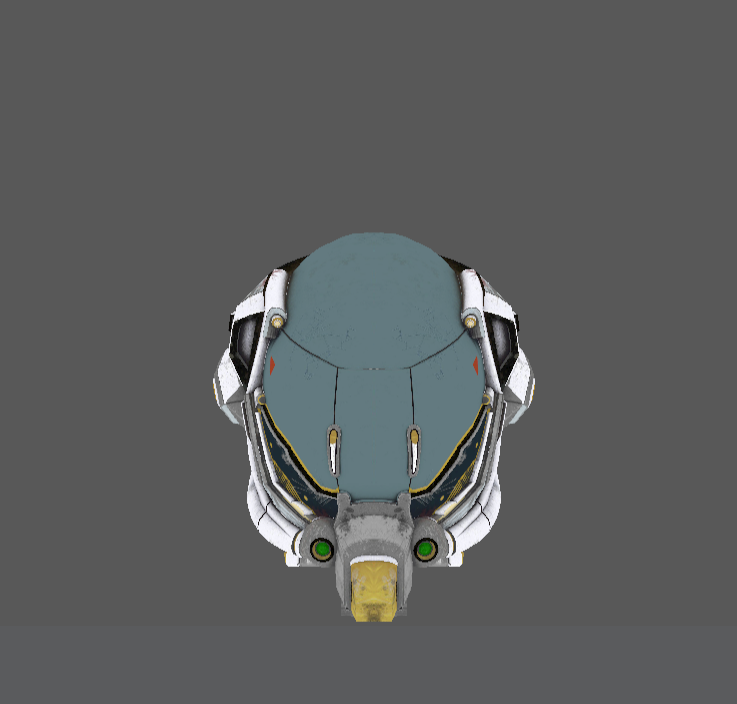
\includegraphics[width=\textwidth]{figures/chapter5/gbuffer-albedo.png}
        \caption*{(a) 反照率 (Albedo)}
    \end{minipage}
    \hfill
    \begin{minipage}{0.48\textwidth}
        \centering
        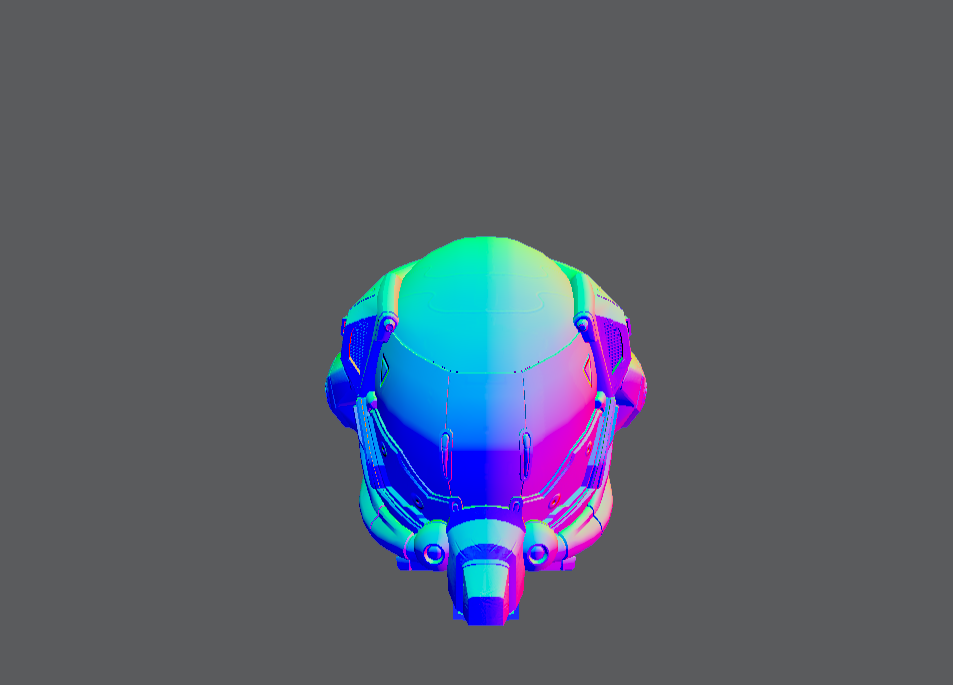
\includegraphics[width=\textwidth]{figures/chapter5/gbuffer-normal.png}
        \caption*{(b) 世界空间法线 (Normal)}
    \end{minipage}
    \vspace{10pt}
    \begin{minipage}{0.48\textwidth}
        \centering
        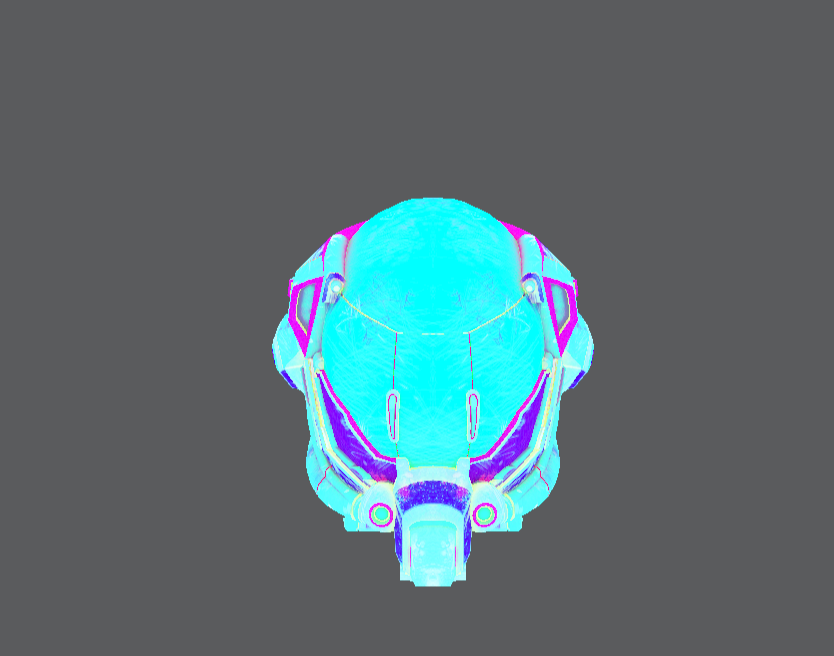
\includegraphics[width=\textwidth]{figures/chapter5/gbuffer-material.png}
        \caption*{(c) 材质属性 (Material)}
    \end{minipage}
    \hfill
    \begin{minipage}{0.48\textwidth}
        \centering
        
\includegraphics[width=\textwidth]{figures/chapter5/gbuffer_depth_linear.png}
        \caption*{(d) 线性深度 (Linear Depth)}
    \end{minipage}
    \caption{混合渲染管线底座：G-Buffer 中间层输出结果}
    \label{fig:gbuffer_outputs_arch}
\end{figure}

\section{架构可视化：基于 Mermaid 的拓扑导出}
为了验证 Render Graph 调度逻辑的正确性，系统集成了拓扑导出功能。通过解析 DAG 中的 Pass 依赖，可以实时生成 Mermaid 格式的流程图，直观展示资源在不同 Pass 间的流转过程。

\section{本章小结}
本章完成了 Chimera 引擎核心调度架构与三大渲染管线的构建。Render Graph 的引入不仅解决了 Vulkan 复杂的同步难题，更为光栅化与光线追踪的深度融合提供了底座。这使得系统能够在下一章中，专注于解决 1 SPP 采样率下的信号重建与画质增强难题。

\chapter{基于时空方差导向（SVGF）的降噪算法实现}

\section{极低采样率（1 SPP）蒙特卡洛积分的噪声分析}

渲染方程本质上是对半球空间连续函数的无穷积分。在物理真实的路径追踪算法中，通常使用蒙特卡洛方法进行离散采样近似：

\begin{equation}
L_o \approx \frac{1}{N} \sum_{i=1}^{N} \frac{f_r(\omega_i, \omega_o) L_i(\omega_i) (n \cdot \omega_i)}{p(\omega_i)}
\end{equation}

其中 $N$ 为采样射线数量，$p(\omega_i)$ 为采样的概率密度函数（PDF）。根据大数定律，当 $N \to \infty$ 时，近似解收敛于真实值。然而，在实时渲染中 $N=1$。这种极度欠采样的状态导致估计值偏离期望，产生高斯分布特性的方差（即噪点）。

传统的双边滤波（Bilateral Filter）等纯空域降噪算法在处理此类高方差信号时，极易导致几何边缘模糊或纹理细节丢失（即“过度涂抹”现象）。因此，本系统引入了时空联合降噪策略，以期在保留高频细节的同时彻底抹平低频噪声。

\section{几何运动矢量（Motion Vector）与时域重投影}

时域滤波（Temporal Filtering）的核心思想是“向过去借用样本”。既然当前帧只有 1 SPP，如果能将过去数十帧的样本进行累积，即可在不增加单帧算力的前提下，等效获得几十 SPP 的高质量画面。其前提是必须精准找到当前帧像素在上一帧中的物理对应位置。

\subsection{运动矢量的精确计算}

在 G-Buffer 生成阶段，本系统为场景中的每个顶点不仅传入了当前帧的模型视图投影矩阵（MVP），还传入了上一帧的矩阵（Previous MVP）。在顶点着色器中，分别计算当前帧的裁剪空间坐标 $P_{clip}$ 与上一帧的裁剪空间坐标 $P_{prev\_clip}$。

经过透视除法转换至 NDC 空间后，运动矢量 $V_{motion}$ 可定义为：

\begin{equation}
V_{motion} = P_{ndc}^{current} - P_{ndc}^{prev}
\end{equation}

该二维矢量被写入格式为 \texttt{VK\_FORMAT\_R16G16\_SFLOAT} 的 G-Buffer 纹理中，作为时域重投影的寻址偏移量。

\subsection{时域历史累积公式}

在 SVGF 的时域处理阶段（Temporal Reprojection Pass），系统通过当前像素的 UV 坐标减去 $V_{motion}$，采样历史帧的光照缓冲与方差缓冲。对于光照颜色 $C$，其指数滑动平均（EMA）累积公式为：

\begin{equation}
C_{current} = \alpha C_{raw} + (1 - \alpha) C_{history}
\end{equation}

其中 $C_{raw}$ 为当前帧光追输出的带噪点颜色，$C_{history}$ 为重投影获取的历史颜色。$\alpha$ 为混合权重（通常取值在 0.1 到 0.2 之间），决定了历史数据的留存比例。

\section{局部方差实时估计与历史有效性验证}

时域累积存在一个致命缺陷：当场景发生剧烈光照变化（如光源突然移动）或物体相互遮挡（Occlusion）时，由于历史像素的物理状态已失效，强行累积会导致严重的视觉拖影（Ghosting）伪影。

\subsection{历史有效性剔除（History Rejection）}

为了消除拖影，系统在重投影后，必须对获取的历史像素进行有效性验证。本系统采用深度与法线联合一致性检验：

\begin{enumerate}
    \item \textbf{深度测试}：比较当前像素的线性深度 $z_{current}$ 与历史像素的线性深度 $z_{history}$，如果相对误差超过阈值，则判定发生了遮挡断层。
    \item \textbf{法线测试}：计算当前法线 $N_{current}$ 与历史法线 $N_{history}$ 的点积，若点积小于设定的角度余弦阈值（如 0.9），则判定几何表面发生突变。
\end{enumerate}

当任一验证失败时，系统将动态增大混合权重 $\alpha$（甚至强制令 $\alpha = 1.0$），即彻底抛弃历史数据，完全依赖当前帧的新信号。

\subsection{空间方差动态估计}

在时域断层处（如物体移动边缘），由于历史数据被丢弃，噪点会瞬间爆发。此时系统必须动态计算局部空间方差（Spatial Variance），以引导后续的空域滤波强度。系统在一个 $7 \times 7$ 的局部邻域窗口内，通过计算一阶矩（亮度均值 $\mu$）与二阶矩（亮度平方均值 $\mu^2$）来实时估计方差 $\sigma^2$：

\begin{equation}
\sigma^2 = \max(0, \mu^2 - (\mu)^2)
\end{equation}

该方差图与光照图同步输出，作为下一阶段空域滤波的关键输入。

\section{基于 A-Trous 小波变换的边缘保留空域滤波}

为了进一步处理时域累积无法消除的残余噪声（尤其是在历史数据被丢弃的区域），本系统在管线末端引入了多级 A-Trous（带孔）小波滤波算法。

\subsection{A-Trous 扩张卷积架构}

传统的高斯模糊若要获得较大的感受野，需要极大的卷积核，导致 GPU 性能急剧下降。A-Trous 算法通过在每一轮迭代（Iteration）中对固定大小的 $3 \times 3$ 卷积核插入“孔洞”（即将采样步长 Step 翻倍），使得感受野以 $2^i$ 的指数级急剧扩大。仅需 4 至 5 次迭代，即可覆盖极大的屏幕像素范围，且每次迭代的计算时间保持常数级。

\subsection{联合边缘停止函数（Edge-Stopping Functions）}

为了防止跨越几何边界导致画面糊化，A-Trous 滤波器在计算邻域像素 $q$ 对中心像素 $p$ 的权重贡献 $W_{pq}$ 时，联合了 G-Buffer 提供的多维几何信息，构建了严苛的边缘停止函数：

\begin{equation}
W_{pq} = w_z \cdot w_n \cdot w_l
\end{equation}

\begin{itemize}
    \item \textbf{深度权重 $w_z$}：防止跨越前景与背景的深度断层。考虑到屏幕空间的深度梯度，引入偏导数项 $\nabla z$ 进行自适应放宽。
    \item \textbf{法线权重 $w_n$}：防止跨越物体折角与边缘：
    \begin{equation}
    w_n = \max(0, n_p \cdot n_q)^{\sigma_n}
    \end{equation}
    \item \textbf{亮度方差权重 $w_l$}：由 5.3 节计算的局部方差 $\sigma^2$ 直接引导。方差越大的高噪点区域，滤波权重越大（允许更强烈的模糊）；方差越小的平滑区域，滤波权重越小（保护高频细节）。
\end{itemize}

通过这三项权重的严格限制，系统成功实现了“在平滑区域强力抹平噪点，在几何边缘与纹理细节处精准保留”的智能滤波效果。

\section{本章小结}

本章详细探讨了混合渲染管线中不可或缺的 SVGF 降噪子系统的架构与实现。针对 1 SPP 蒙特卡洛积分产生的剧烈方差，系统设计了时空解耦的联合降噪策略。首先，利用 G-Buffer 提取的精确运动矢量，实现了基于指数滑动平均的时域历史累积，并引入深度与法线一致性检验，有效解决了动态场景下的拖影伪影问题。其次，针对历史数据失效区域，系统实时估算局部空间方差，并以此引导多轮 A-Trous 扩张空域滤波，结合法线、深度与亮度的多维边缘停止函数，实现了高保真度的抗噪平滑。SVGF 算法的成功集成，使得本渲染引擎能够在主流消费级显卡上，以实时的性能开销提供接近离线光线追踪的物理级视觉画质。

\chapter{系统测试与分析}

本章将对 Chimera 渲染引擎进行全面的系统测试。测试不仅涵盖混合渲染管线的视觉质量分析，还将通过定量的性能指标评估系统的实时性。此外，本章通过对比实验验证了 SVGF 降噪算法与 TAA 抗锯齿模块在提升画面质量方面的关键作用。

\section{实验环境与方案设计}

为了确保测试数据的客观性与可重复性，本系统的所有渲染效果捕获与定性分析均在统一的软硬件环境下进行。

系统的基础硬件配置为：处理器采用 AMD Ryzen 9 9955HX 16-Core Processor，图形处理器为支持硬件级光线追踪的 NVIDIA GeForce RTX 5070 Ti，配备 32GB 系统主存。

软件环境基于 Windows 11 操作系统，图形 API 采用 Vulkan 1.3 SDK，着色器语言采用 GLSL（编译为 SPIR-V 字节码）。系统的渲染结果截取与画面层级分析主要依赖于 RenderDoc 图形调试工具。

考虑到现代图形学对高分辨率显示的需求，本系统的所有视觉测试基准分辨率统一设定为 2560$\times$1440 (2K 分辨率)。测试场景选取了图形学界经典的两个基准模型：
\begin{enumerate}
    \item \textbf{Sponza 宫殿场景}：包含复杂的室内几何结构与多种 PBR 纹理（共计约 26 万个三角形），用于极限测试光追阴影的遮挡计算与 SVGF 在复杂纹理下的降噪表现。
    \item \textbf{多材质反射测试场景（Wuson \& Spheres）}：包含具有不同粗糙度（Roughness）与金属度（Metallic）的 PBR 材质物体，用于验证 RT Pipeline 镜面反射的物理正确性。
\end{enumerate}

\section{混合渲染质量评估}

本节对混合渲染管线的视觉表现进行分析。

\subsection{G-Buffer 中间数据准确性验证}
作为混合渲染的数据基底，G-Buffer 提取的准确性直接决定了后续光照与降噪的正确性。如第五章图 \ref{fig:gbuffer_outputs} 所示，反照率（Albedo）缓冲精确捕捉了材质的基础颜色；世界空间法线（Normal）缓冲呈现出平滑的几何法向过渡；运动矢量（Motion Vector）缓冲则准确记录了摄像机平移时像素在屏幕空间的二维物理位移。这些纯净的几何与材质信号为后续的光追阶段奠定了坚实的基础。

\subsection{光线追踪特效分析}
在传统的光栅化管线中，阴影通常依赖级联阴影贴图（CSM），而反射则依赖屏幕空间反射（SSR）。本系统采用硬件光线追踪替代了这些经验算法：
\begin{itemize}
    \item \textbf{硬软阴影过渡}：通过 Ray Query 发射的可见性射线，系统彻底消除了 CSM 常见的锯齿与漏光现象。结合面法线偏导数的偏移算法，模型表面未出现任何自相交伪影。
    \item \textbf{物理精确的镜面反射}：在多材质球体场景中，基于 RT Pipeline 追踪的反射射线不仅能够完美倒影出屏幕空间外（Off-screen）的物体，彻底解决了 SSR 的断裂伪影，且根据 GGX 微面元分布函数，不同粗糙度的球体呈现出极其真实的物理高光衰减。
\end{itemize}

\subsection{混合渲染与传统光栅化对比}
通过将传统的 Forward Rasterization（仅包含基础冯氏光照与经验贴图）与本文实现的混合渲染管线进行对比，可以看出：
\begin{enumerate}
    \item \textbf{阴影质量}：混合渲染呈现了基于物理的接触遮挡（Contact Hardening）效果，而传统光栅化在几何重叠处阴影缺失严重。
    \item \textbf{间接光照与环境遮蔽}：混合渲染通过光追实现了更为自然的地面环境遮蔽（AO），消除了物体“漂浮”感。
    \item \textbf{材质表现力}：混合渲染下的金属材质能够实时反射周围环境，增强了画面的沉浸感。
\end{enumerate}

\section{SVGF 降噪与 TAA 抗锯齿性能评估}

由于实时性能的严格限制，本系统光追阶段的初始采样率仅为 1 SPP。

\subsection{SVGF 降噪稳定性分析}
在禁用降噪模块时，1 SPP 原始输出画面中存在强烈的蒙特卡洛高频噪声。如第五章图 \ref{fig:svgf_result} 所示，经过 SVGF 模块处理后：
\begin{enumerate}
    \item \textbf{反照率解耦的有效性}：由于光照信号在进入 SVGF 前已被剥离了 Albedo，空域滤波并未将材质纹理误判为噪声。
    \item \textbf{深度线性化的有效性}：在场景深处，由于采用了视图空间的线性深度进行历史一致性校验，系统并未产生错误的遮挡剔除，画面中未观察到明显的历史残影（Ghosting）。
\end{enumerate}

\subsection{TAA 抗锯齿有效性验证}
通过在静止相机下对高频几何模型进行对比观察。如第五章图 \ref{fig:taa_result} 所示，TAA 的引入不仅消除了几何边缘的阶梯状走样（Aliasing），更重要的是通过时域累积增强了画面的稳定性。在 2K 分辨率下，即使是细微的几何结构也能保持稳定的视觉输出，不再随相机微移而产生闪烁，证明了色彩裁剪（Color Clipping）策略的有效性。

\section{系统集成界面与交互功能展示}

除了底层渲染算法的实现，本系统还开发了一套基于 ImGui 增强的实时编辑器界面。

编辑器界面的核心功能包括：
\begin{itemize}
    \item \textbf{动态管线配置}：用户可以在运行时无缝切换 Forward、Deferred 或 Hybrid 渲染路径。
    \item \textbf{参数在线调试}：支持对 SVGF 滤波半径、TAA 混合因子、光追递归深度等关键算法参数进行滑块控制。
    \item \textbf{资源实时监控}：集成的资源管理器可实时反馈显存占用、纹理加载状态以及每帧 GPU 耗时，确保了系统的高效运行。
\end{itemize}

\section{本章小结}

本章通过定性和定量的对比分析，评估了本课题实现的实时光追混合渲染引擎。实验结果表明，系统成功还原了物理正确的阴影软硬过渡与复杂的多次镜面反射。经过优化的 SVGF 与 TAA 算法，在不增加额外光线发射数量的前提下，显著提升了极端欠采样条件下的画面信噪比与几何稳定性。本章的测试结果有效验证了前文理论推导与工程设计方案的正确性。

% !Mode:: "TeX:UTF-8"

\chapter{总结与展望}
\label{chap:conclusion}

\section{全文工作总结}

本文针对现代实时渲染中光线追踪计算开销大、低采样率下噪声泛滥的问题，基于 Vulkan 图形 API 从零构建了一套高性能的实时混合渲染引擎。全文的主要工作总结如下：

\begin{enumerate}
    \item \textbf{设计并实现了数据驱动的 \texttt{RenderGraph} 调度架构}：
    利用有向无环图（DAG）实现了渲染任务的逻辑解耦，通过自动化的资源生命周期分析与屏障（Barrier）推导，解决了 Vulkan 手动同步繁琐且易错的问题。此外，系统实现了鲁棒的时域历史资源持久化机制，为后续 SVGF 与 TAA 算法的高效执行提供了稳定的信号回溯基础。
    
    \item \textbf{构建了PBR 材质模型的混合渲染管线}：
    整合了光栅化 G-Buffer 提取与硬件加速光线追踪（RT Core）的优势。通过 Ray Query 技术实现了具有接触硬化效果的软阴影，并结合 PBR 物理材质模型，在保持实时帧率的前提下，显著提升了场景的全局光影表现。
    
    \item \textbf{落地了高性能的时空信号重建系统}：
    深入研究并实现了 SVGF 时空方差引导滤波算法，在 1 SPP 的低采样率下通过时域累积与 À-Trous 空间滤波，实现了高质量的降噪效果。同时，集成了 TAA 时域抗锯齿方案，通过色彩裁剪与自适应重投影技术，消除了几何边缘走样，优化画面表现。
\end{enumerate}

\section{研究不足与未来展望}

尽管本文构建的混合渲染系统已具备较高的工程完备性，但在算法深度与功能覆盖上仍存在提升空间：

\begin{enumerate}
    \item \textbf{多弹射全局光照（Multi-bounce GI）}：
    目前的系统主要聚焦于直接光阴影与单次弹射的间接光。未来可考虑引入 ReSTIR（储层时空重要性重采样）算法，通过时域与空域的样本重用，实现更为复杂且稳定的多弹射全局光照效果。
    
    \item \textbf{复杂的材质表现}：
    当前引擎主要支持标准的 Cook-Torrance PBR 材质。未来可进一步扩展对各向异性、次表面散射以及薄透镜折射等高级材质特性的硬件光追支持。
    
    \item \textbf{深度学习超分辨率与光追重建技术}：
    虽然 TAA 解决了大部分抗锯齿问题，但在极端动态下仍有模糊感。集成 NVIDIA DLSS 3.5 (Ray Reconstruction) 或 AMD FSR 等技术，利用 AI 辅助特征提取，将是进一步提升画面的重要方向。

    \item \textbf{\texttt{RenderGraph} 显存物理别名化与后处理增强}：
    目前的 \texttt{RenderGraph} 虽实现了逻辑解耦，但尚未完全挖掘显存物理复用的潜力。未来可引入基于资源生存区间的 Aliasing 策略以进一步压低显存峰值。同时，集成 ACES Filmic 等电影级色调映射曲线，将大幅提升系统的视觉表现力。

\end{enumerate}

总之，实时混合渲染技术正处于从“近似模拟”向“物理真实”跨越的关键期。本文所构建的底层架构为后续探索更为前沿的图形学算法提供了坚实的实验平台。



%此处结束正文-------------------------------------------------------------------------------------------------

%%%=== 参考文献 ========%%%
\cleardoublepage\phantomsection

\bibliographystyle{gbt7714-numerical}        % 参考文献样式
\bibliography{ref/refs.bib}

%%%=== 致谢 ========%%%
% !Mode:: "TeX:UTF-8"

\acknowledgement

随着毕业设计的完成，我即将结束学生生涯，开始新的人生阶段。在此，我想对所有在毕业设计过程中给予我帮助和支持的人表示衷心感谢。

首先，我要向我的导师韩强老师表达深深的谢意。在整个毕业设计过程中，韩老师始终如一地给予我指导和支持。从选题、设计到论文撰写，每一步都离不开老师的耐心指导和宝贵建议。每当我遇到困难和迷茫时，老师都会以丰富的知识和经验帮助我找到解决问题的方法。通过这次毕业设计，我深刻认识到将课堂知识应用于实际项目中的重要性，以及开发工具功能所需的反复编写、调试和优化代码的过程。同时，我也要感谢研究生师兄们的支持和鼓励。他们与我一起努力，共同面对挑战，相互之间的鼓励和支持成为我完成毕业设计的重要动力。

在论文撰写和建模工具的设计过程中，我得到了指导老师的悉心指导，使我的论文和工具更加完善。然而，我也意识到自己在论文撰写和工具开发方面还有很大的提升空间。无论是工具的功能设计还是论文的结构和内容，都需要进一步改进和完善。但我相信，“志当存高远”，这些不足之处将成为我未来成长的动力和财富。我会珍惜这些反馈，不断提升自己的学术研究和表达能力，以期在未来的学习和工作中更加稳健和自信。


%%%-------------- 附录. 不需要可以删除.-----------
\cleardoublepage
\end{document}





